\documentclass[12pt]{report}
\usepackage{semtrans}
\usepackage{graphicx}
\usepackage{tabularx}
\usepackage{longtable}
\usepackage{ltxtable}
\usepackage[utf8]{inputenc}
\usepackage[Glenn]{fncychap}
\usepackage{ltablex}
\usepackage[T1]{fontenc}
\usepackage{enumitem}
\usepackage[margin=2cm]{geometry}
\usepackage{array}
\usepackage[table]{xcolor}
\usepackage{pdfpages}
\usepackage{appendix}
\usepackage{newclude}
\usepackage{titling}
\usepackage[cc]{titlepic}
\usepackage{hyperref}
\usepackage{wrapfig}
\usepackage{caption}
\usepackage{subcaption}
\usepackage[nonumberlist]{glossaries}
\usepackage{float}
%\usepackage{titlesec}


%\titleformat*{\subsubsection}{0.4em}
%\titleformat*{\subparagraph}{0.3em}


\hypersetup{
    colorlinks=false,
    pdfborder={0 0 0},
}
\newcommand{\subtitle}[1]{%
  \posttitle{%
    \par\end{center}
    \begin{center}\large#1\end{center}
    \vskip0.5em}%
}

\makeatletter
\renewcommand*{\@makechapterhead}[1]{%
  \vspace*{10\p@}%
  {\parindent \z@ \raggedright \normalfont
    \ifnum \c@secnumdepth >\m@ne
      \if@mainmatter%%%%% Fix for frontmatter, mainmatter, and backmatter 040920
        \DOCH
      \fi
    \fi
    \interlinepenalty\@M
    \if@mainmatter%%%%% Fix for frontmatter, mainmatter, and backmatter 060424
      \DOTI{#1}%
    \else%
      \DOTIS{#1}%
    \fi
  }}
% For the case \chapter*:
\renewcommand*{\@makeschapterhead}[1]{%
  \vspace*{10\p@}%
  {\parindent \z@ \raggedright
    \normalfont
    \interlinepenalty\@M
    \DOTIS{#1}
    \vskip 40\p@
  }}
\makeatother

\newcommand{\sprintPrefix}[0]{$\cdot$ }
%\dateFormat{month}{day}{year}{delimiter}
%\newcommand{\dateFormat}[4]{#1#4#2#4#3}
%\newcommand{\dateFormat}[4]{#2#4#1#4#3}
\newcommand{\dateFormat}[3]{#3.#1.#2}
\newcommand{\JIRA}[1]{\\JIRA reference: #1}
\newcommand{\JIRAS}[1]{(#1)}
\newcommand{\SP}[1]{(#1 SP)}
\newcommand{\highlight}[1]{\textsc{#1}}

\makeglossaries
\newglossaryentry{kds}{name=SDK, description={Software Development Kit}}
\newglossaryentry{ascii}{name=ASCII, description={American Standard Code for Information Interchange}}
\newglossaryentry{ca}{name=CA, description={Certificate Authority}}
\newglossaryentry{ldia}{name=AIDL, description={Android Interface Definition Language}}
\newglossaryentry{ipc}{name=IPC, description={Inter-process communication}}
\newglossaryentry{cpu}{name=CPU, description={Central Processing Unit}}
\newglossaryentry{jndk}{name=JNDK, description={Java Native Development Kit}}
\newglossaryentry{nato}{name=NATO, description={North Atlantic Treaty Organization}}
\newglossaryentry{sp}{name=sp, description={Scale independent pixels}}
\newglossaryentry{cots}{name=COTS, description={Commercial off-the-shelf}}
\newglossaryentry{mb}{name=MB, description={Megabyte}}
\newglossaryentry{sms}{name=SMS, description={Short Message Service}}
\newglossaryentry{id}{name=ID, description={Identification/Identity/Identifier}}
\newglossaryentry{stanag}{name=Stanag 4406, description={The NATO standard for Military Messaging based on X.400}}
\newglossaryentry{smtp}{name=SMTP, description={"Simple Mail Tranfer Protocol" defined by RFC 5321}}
\newglossaryentry{ip}{name=IP, description={"Internet protocol" defined by RFC 791}}
\newglossaryentry{pami}{name=IMAP, description={"Internet message access protocol" defined by RFC 3501}}
\newglossaryentry{it}{name=IT, description={Information Technology}}
\newglossaryentry{git}{name=Git, description={Distributed version control system}}
\newglossaryentry{github}{name=GitHub, description={Web-based hosting service}}
\newglossaryentry{ide}{name=IDE, description={Integrated development environment}}
\newglossaryentry{osx}{name=OS X, description={A series of Unix-based graphical interface operating systems}}
\newglossaryentry{xml}{name=XML, description={Extensible Markup Language}}
\newglossaryentry{maven}{name=Maven, description={A build automation tool typically used for Java projects}}
\newglossaryentry{svn}{name=SVN, description={"SubVersion", centralized version control}}
\newglossaryentry{pop}{name=POP3, description={"Post Office Protocol, version 3" defined by RFC 1081}}
\newglossaryentry{ssl}{name=SSL/TLS, description={"Secure sockets layer/transport layer security" defined by RFC 6101 and RFC 5246}}
\newglossaryentry{ssl1}{name=SSL, description={"Secure sockets layer" defined by RFC 6101 and RFC 5246}}
\newglossaryentry{tls}{name=TLS, description={"Transport layer security" defined by RFC 6101 and RFC 5246}}
\newglossaryentry{tcp}{name=TCP, description={"Transmission Control Protocol" first specified by RFC 675}}
\newglossaryentry{emims}{name=S/MIME, description={"Secure/Miltipurpose Internet Mail Extensions", defined by RFC 3369, RFC 3370, RFC 3850 and RFC 3851}}
\newglossaryentry{mime}{name=MIME, description={"Multipurpose Internet Mail Extensions", defined by RFC 2045, RFC 2046, RFC 2047, RFC 4288, RFC 4289 and RFC 2049}}
\newglossaryentry{ocsp}{name=OCSP, description={"Online Certificate Status Protocol", defined by RFC 2560}}
\newglossaryentry{ldap}{name=LDAP, description={"Lightweight Directory Access Protocol", defined by RFC 4511}}
\newglossaryentry{ndk}{name=NDK, description={Native Development Kit}}
\newglossaryentry{sl}{name=SL4A, description={Scripting Layer for Android}}
\newglossaryentry{api}{name=API, description={Application programming interface}}
\newglossaryentry{php}{name=PHP, description={Hypertext Preprocessor}}
\newglossaryentry{vm}{name=VM, description={Virtual machine}}
\newglossaryentry{json}{name=JSON, description={JavaScript Object Notation}}
\newglossaryentry{xsd}{name=XSD, description={XML Schema Definition}}
\newglossaryentry{jvm}{name=JVM, description={Java Virtual Machine}}
\newglossaryentry{jdk}{name=JDK, description={Java Development Kit}}
\newglossaryentry{jar}{name=JAR, description={Java ARchive}}
\newglossaryentry{cvs}{name=CVS, description={Concurrent Versions System}}
\newglossaryentry{pbe}{name=PBE, description={Password Based Encryption}}
\newglossaryentry{pbkdf}{name=PBKDF2, description={Password-Based Key Derivation Function 2}}
\newglossaryentry{osi}{name=OSI, description={Open Systems Interconnection}}
\newglossaryentry{rfc}{name=RFC 5321, description={Definition of SMTP}}
\newglossaryentry{rfc4}{name=RFC 4409, description={Definition of a mail submission agent (MSA)}}
\newglossaryentry{rfc5}{name=RFC 5322, description={Definition of Internet Message Format}}
\newglossaryentry{rfc2}{name=RFC 2156, description={Definition of Mime Internet X.400 Enhanced Relay.  A mapping between X.400 and RFC 822/MIME}}
\newglossaryentry{rfc6}{name=RFC 6477, description={Definition of Registration of Military Message Handling System (MMHS)}}
\newglossaryentry{gps}{name=GPS, description={Global Positioning System}}
\newglossaryentry{gui}{name=GUI, description={Graphical User Interface}}
\newglossaryentry{ui}{name=UI, description={User Interface}}
\newglossaryentry{aes}{name=AES, description={Advanced Encryption Standard}}
\newglossaryentry{cbc}{name=CBC, description={Cipher-Block Chaining}}
\newglossaryentry{essiv}{name=ESSIV, description={Encrypted salt-sector initialization vector}}
\newglossaryentry{sha}{name=SHA256, description={Secure Hash Algorithm}}
\newglossaryentry{css}{name=CSS, description={Cascading style sheets, RFC 2318}}
\newglossaryentry{jpeg}{name=JPEG, description={Joint Photographic Experts Group}}
\newglossaryentry{pbsha}{name=PBKDF2 HMAC-SHA1, description={Password-Based key Derivation Function 2}}
\newglossaryentry{netb}{name=NetBeans, description={An open-source software development project with an active community of collaborating users and developers}}
\newglossaryentry{uml}{name=UML, description={Unified Modeling Language}}
\newglossaryentry{essiv2}{name=ESSIV:SHA256, description={Encrypted sector|salt initial vector where sha256 is a hash algorithm}}
\newglossaryentry{k9m}{name=K-9 Mail, description={Evaluation criteria - open source email client for Android}}
\newglossaryentry{x5}{name=X509Tools, description={..}}
\newglossaryentry{r2m2}{name=R2Mail2, description={An email client for Android OS}}
\newglossaryentry{ips}{name=IPSec, description={Internet Protocol Security}}
\newglossaryentry{imapi}{name=IMAPIdle, description={An optional expansion of the IMAP email accessing protocol that allows the server to send new message updates to the client in real time}}
\newglossaryentry{idle}{name=IDLE, description={An integrated development environmentfor Python}}
\newglossaryentry{ant}{name=Ant, description={Java library to build packages}}
\newglossaryentry{xs}{name=XStream, description={Parsers libraries and tools - a simple library to serialize objects to XML and back again}}
\newglossaryentry{jrock}{name=JRockit, description={A proprietary Java Virtual Machine}}
\newglossaryentry{ieee829}{name=IEEE829, description={The 829 Standard for Software and System Test Documentation}}
\newglossaryentry{junit}{name=Junit, description={A unit testing framework for the Java programming language}}
\newglossaryentry{acid}{name=ACID, description={Atomicity, consistency, isolation, durability}}
\newglossaryentry{bouncy}{name=BouncyCastle, description={Java Cryptography Library}}
\newglossaryentry{spongy}{name=SpongyCastle, description={Repackage of \gls{bouncy} for Android}}
\newglossaryentry{dpi}{name=dpi, description={Dots per inc, a measure of screen density}}
\newglossaryentry{mmhs}{name=MMHS, description={Military Message Handling System, described by RFC6477}}
\begin{document}
\setlength{\parindent}{0in}

\renewcommand{\thepage}{\roman{page}}

\title{XOXOmail}
\subtitle{Formal and secure messaging on a mobile platform}

\titlepic{
\begin{figure}[h!]
\begin{center}

\includegraphics[scale=0.7]{noshadow1}
\end{center}
\end{figure}}

\author{Formal and secure messaging on a mobile platform\\ \\ \\  Lars Smørås Høysæter \\ Aleksander Aas Sjåfjell \\ Ida Katrine Børstad Thoresen \\ Kristin Tønnesen\\ Magnus Hertzberg Ulstein \\ Nicklas Sørlie Utgaard}



\maketitle
\clearpage



\chapter*{Abstract}

\textbf{This report} addresses the problem of communicating with the XOmail system from a mobile device. XOmail is a mail service that focuses on security and on getting the mail to its destination in a short time. During the project we created an Android application for cell phones and other devices that could provide the same security and stability as XOmail does on computers. The biggest issue of the project was how to make a handheld device secure enough to send important messages and to develop a user interface that is customized for small screens and easy to use. 
\newline
\newline
\textbf{The motivation} for working on this task is that even if there are a lot of different email applications for handheld devices today, none of them support the amount of security we need. The newest and most exciting part of the assignment was figuring out how to implement the required level of security. In addition, none of us have done extensive work with the Android framework before, so we are eager to learn more about the technology. Android applications are the new hot stuff in the development departments today, so getting the opportunity to learn about the newest products on the market is very interesting. 
\newline
\newline
\textbf{The demands} of our software project are, at first glance, quite simple. By implementing a mobile version of XOmail, the XOXOmail client, we will show what a working client might look like. It is important to note that we will focus on creating a proof-of-concept messaging client that uses the standards given by Thales. The primary focus is not on creating a fancy user interface, but rather on fulfilling the needs of the users. 
\newline
\newline
\textbf{The results} of this project will be unveiled as soon as the project has ended. It is, at this time, quite difficult to say anything about the results.



\chapter*{Preface}

This report was written for a project in the course TDT4290 Customer Driven Project at Norwegian University of Technology and Science (NTNU). The project was executed on behalf of Thales Norway AS between the 21th of August and the 22th of November.
\newline
\newline
The project team consisted of six students from the Department of Computer and Information Science at NTNU. Our task was to develop a mail application for handheld devices that could communicate with Thales' existing XOmail server.
\newline
\newline
The team would like thank our advisor Mohsen Anvaari for his advice and help throughout the project. We would also like to thank Reidar Conradi for his feedback. 
\newline
\newline
In addition we would like to thank our customer Thales and their contact persons Christian Tellefsen and Stig Bjørlykke. Their input and feedback have been invaluable and we would like to thank them for the cooperation. 
\newline
\newline
We would also like to thank the persons that set aside the time to participate in our usability tests and give us their valuable feedback about the design and usability of the XOXOmail application.


\tableofcontents

\listoffigures

\listoftables

\chapter*{Detailed contents}

\section*{Goal of the report}
This report documents the entire process behind developing the application. It describes what was done, why it was done and when it was done. The report contains summaries of all the pre-studies the group has been doing throughout the project, as well as the decisions made. It will describe the reason behind the actions and decisions. The report can also be used to monitor the development process of making the application the customer wants. In short, it describes how the prioritizations was made, and sums up what went well and what went not so well during the project.

\section*{What this report covers}
Chapter 2 - Project directive describes all the involved parties in this project. \\ 
Chapter 3 - Project planning gives an overview of how this task have been planned, how the team
\hspace*{5.5em}is organized and the quality assurance measures of the project. \\
Chapter 4 - Preliminary studies gives summaries of all the preliminary studies done in this project,
\hspace*{5.5em}as well as the decisions that have been made. \\
Chapter 5 - Requirements contains user stories and business requirements that detail how the
\hspace*{5.5em}application should look and behave. \\ 
Chapter 6 - Test plan explains how the code have been tested in this project. \\
Chapter 7 - Architectural description describes the architecture of the application, both backend
\hspace*{5.5em}and frontend. \\
Part II - Scrum process describes all of the sprints very carefully. It also includes the product
\hspace*{4.5em}backlog and the changelog. \\
Part III - Conclusion \& Reflection includes reflections on how the team has worked together, and
\hspace*{4.5em}describes disputes and agreements.

\section*{How this report is structured}
The report is divided into parts as well as chapters. This gives a much better overview of the report, and makes it a lot easier to find your way around it. It is divided into four parts; planning, preliminary studies, sprints and reflection.

\renewcommand{\thepage}{\arabic{page}}
\setcounter{page}{1}

\part{Planning \& Requirements}

%\chapter{Introduction}

	\chapter{Introduction}

This chapter is a technical introduction to the project. The purpose of this chapter is to give an overview of the task to be solved and the most important terms used in the report.

\subsection*{The existing product}
Thales has developed an information handling and transfer system called XOmail \cite{bib:xomail}, which has been in operational use for more than 20 years. In many ways, it could be compared to a regular, well-known email system. The first and biggest difference between regular email and and XOmail is that XOmail is developed with large formal organizations and military messaging procedures in mind. This is the reason why Thales has been delivering XOmail as a complete product to several European \gls{nato} member countries.  
\newline
\newline
The messages that are sent are defined to have a security label, which is a declaration of the required clearance level the receivers must have. The security label specifies that only people or groups with the required (or higher) security clearance can see the messages. Security is an important feature of XOmail, and it has never lost a message in 20 years of operation. 

\subsection*{What Thales wants us to make}
Thales’ existing product is a complete messaging platform for messaging in large organizations, but the current system is primarily made for use on typical computers with relatively large screens. What Thales wants to know is if it is possible to create a mobile messaging platform building on the existing infrastructure already in use by XOmail. It is important to note that this mobile platform will only have a subset of the functions that the original system has and the main focus is on security, efficiency and ease of use.
\newline
\newline
Since Thales has not tried to implement XOmail on mobile platforms, there is no existing framework to start with. Thales wants a prototype that demonstrates a possible solution to their problem. Security is of great importance, but the main focus should be on implementing functionality that is critical for showing the concept software.  
\newline
\newline
Even though XOmail primarily targets the military and other large organizations where security and security declarations are important, it is important to keep in mind that this software also should be well suited for other groups or organizations that have a need for a user-friendly portable system for sending urgent messages. A few of the possible candidates include paramedics, security firms and joint civilan-military operations or exercises.
\newline
\newline
For a summary of what Thales already has and what they want, see table \ref{tab:introcomparison} at page \pageref{tab:introcomparison}.

\subsection*{A short overview of the standards of XOmail}
XOmail is based on the \gls{nato} military messaging standard \gls{stanag}. This standard is used for both Strategic and Tactical messaging \cite{bib:stanag}. It has a number of special protocols used to support tactical messaging to support links with very low bandwidth.
\newline
\newline
The standard is based on binary encoded data, and there are limited libraries freely available for these protocols. Special attributes like information sensitivity and priority are defined by extensions to the Internet Mail RFCs. Our connection to Thales’ system goes through a XOmail \gls{smtp} gateway. \gls{smtp}, which is shorthand for Simple Mail Transfer Protocol \cite{bib:smtp}, is an Internet standard for electronic mail transmission over \gls{ip} networks. Messages to other users are sent by sending an email to the server with an address, and then the server handles the message headers and other important attributes. The messages are then pushed to the correct recipients via \gls{pami} \cite{bib:imap}, which is an abbreviation for Internet Message Access Protocol, and is one of the most prevalent Internet standard protocols for email retrieval. 

\begin{tabular}{l|l}
What Thales has&What Thales wants\\ \hline
An information handling and transfer system developed for large formal organizations and military messaging procedures&A system for handheld devices with a subset of the existing functions\\ \hline
A large number of ways of giving a message attributes&Focus on security label, priority and type\\ \hline
Extensive focus on security and reliability&Focus on security and usability\\ \hline
Support for a broad range of attachments&Support for images, text and video\\ \hline
\caption{Thales' current and wanted situation}
\label{tab:introcomparison}
\end{tabular}


%\chapter{Project directive}

	\chapter{Planning}

This chapter is about how we planned our project. The purpose of this chapter is to explain how our team is organized, who we are, why we do this project and how do it.

\section{Overall project plan}

\subsection{Project name}
XOXOmail

\subsection{Project sponsor}

The customer for this project is Thales Norway AS. Thales is a leading international electronics and systems group, focusing on defense, aerospace and security markets worldwide. The cutting edge technology in use at Thales offers capabilities unmatched in Europe for the development and deployment of mission-critical information systems proven in the field. The group’s civil and military business areas develop in parallel and share a common base of technologies to serve a single objective: the security of people, property and nations.
\newline
\newline
After Thales’ 50 years of industrial activity in Norway it is now one of Norway’s largest industrial centers of expertise for mission-critical IT and telecommunications solutions and one of the principal supplies of military communication systems to the Norwegian Armed Forces. [1]
\newline
\newline
See table \ref{tab:customer} at page \pageref{tab:customer}
\begin{table}
\begin{tabular}{l|l|l|l}
\textbf{Name} & \textbf{Office} & \textbf{Phone nr} & \textbf{E-mail} \\ \hline \hline
Sølve Conradi Olsen & Thales Norway & 907 80 179 & solve.olsen@thalesgroup.com \\ hline
Christian Tellefsen & Thales Norway & 959 98 765 & christian.tellefsen@thalesgroup.com \\ hline
Stig Bjørlykke & Thales Norway & 982 29 806 & stig.bjorlykke@thalesgroup.com
\end{tabular}
\caption{The customer representatives} \label{tab:customer}
\end{table}

\subsection{Involved Parties}

In this project there are only three involved parties: a) the customer b) the project team and c) the advisor. The customer, Thales, described in the section above was represented by Christian Tellefsen and Stig Bjørlykke. The project team consists of 6 students from the Department of Computer and Information Science (IDI) at the Norwegian University of Science and Technology (NTNU).The advisor was Mohsen Anvaari who was assigned to our team to guide and help us during the project period.
\newline
\newline
See table \ref{tab:projectgroup} at page \pageref{tab:projectgroup}
\begin{table}
\begin{tabularx}{\linewidth}{>{\setlength\hsize{.52\hsize}}X|>{\setlength\hsize{0.5\hsize}}X|>{\setlength\hsize{.3\hsize}}X|>{\setlength\hsize{.5\hsize}}X}
\textbf{Name} & \textbf{Address} & \textbf{Phone nr} & \textbf{E-mail} \\ \hline \hline
Ida Thoresen & Klæbuveien 143, 7031 & 936 68 688 & idakatt@stud.ntnu.no\\ \hline
Kristin Tønnesen & Lars Onsagersvei 12, 7030 & 986 28 958 & kristonn@stud.ntnu.no \\ \hline
Lars Høysæter & Innherredsveien 2a, 7014 & 900 31 814 & larssmor@stud.ntnu.no\\ \hline
Nicklas Utgaard & Odd Brochmanns veg 47, 7030 & 976 87 790 & nicklau@stud.ntnu.no\\ \hline
Magnus Ulstein & & 472 31 418 & magnuul@stud.ntnu.no\\ \hline
Aleksander Sjåfjell & Odd Brochmanns veg 60, 7030 & 456 01 212 & aleksasj@stud.ntnu.no
\end{tabularx}
\caption{The project group} \label{tab:projectgroup}
\end{table}

See table \ref{tab:advisor} at page \pageref{tab:advisor}
\begin{table}
\begin{tabular}{l|l|l|l}
\textbf{Name} & \textbf{Work} & \textbf{Phone nr} & \textbf{E-mail} \\ \hline \hline
Mohsen Anvaari & PhD-stud. NTNU & 405 70 403 & mohsena@idi.ntnu.no
\end{tabular}
\caption{Our advisor} \label{tab:advisor}
\end{table}

\subsection{Background for the project}

This project was given to us as an assignment in the course TDT4290 Customer Driven Project. Since the society is constantly changing, the technology must follow along with the enormous changes we see today. Because of these changes Thales found that they needed a handheld android version of their existing XOmail system. This new handheld system would help the users of XOmail so that they could also use it in the field and not only at the office. When able to use this mailing system not only in contact with a computer, the regular working day of Thales customers would be a lot easier, especially since their primary customer is the Norwegian military.

\subsection{Measurement of project effects}

Thales has proposed the following effects:
\begin{itemize}
\item{}Test user interface for message-based communication on a handheld device.
\item{}Make a prototype that can give inspiration for further product development and be used as a demonstration internally and to customers.
\end{itemize}

\newpage
\subsection{General terms}

\subsubsection{Technical Limitations}

\paragraph{Android}
Android is a quite new platform and none of us have been doing much programming in it before starting on this project. So learning how Android works and finding technical tools that Android supports is going to be a time consuming task. We will develop our project in Android version 2.2 with API level 8. The reason for choosing this version of Android is that we do not want to depend on features that only exist in the newer versions of Android. 

\paragraph{Screen}
The mail client will be used on devices with relatively small touch screens which means that the application must be carefully designed to accommodate the limited size. In addition we need to put a lot of thought into the design so that it becomes easy to use. The application must be designed to scale well with different screen resolutions.

\subsubsection{Non-technical Limitations}

\paragraph{Language}
The entire project is to be delivered in English, so we all have to write in our second language. This means that the report work will take more time than writing in Norwegian. 

\paragraph{Time}
We have a set timeframe of 13 weeks with a delivery deadline that cannot be changed. This gives us a set amount of time and we probably do not have the time to implement all parts of the application. We have to focus on the parts we find most important. The specified timeframe gives us challenges when it comes to planning and priorities of the different tasks.

\subsubsection{Tool Selection}

\paragraph{Git \& GitHub}
Git is an extremely fast, efficient and distributed version control system ideal for the collaborative development of software. It can be used to manage all your public and private repositories, and makes it easy to share and work with the same source code and documents [9]. GitHub is a hosting system that implements git and is free to use if you choose to share your source code with others. 

\paragraph{Google Docs}
Google Docs is a free web based service that offers users the ability to create and edit documents online. Google Docs lets us share documents easily and collaborate on the same document simultaneously.    

\paragraph{NetBeans IDE}
NetBeans IDE is an integrated development environment for developing with Java. It is written in Java and can run on Windows, Linux and OS X. NetBeans IDE is one of the most popular IDEs. Using a common IDE helps speed up the development process.

\paragraph{Apache Maven}
Maven is a build automation tool which is typically used with Java projects. It uses an XML file to describe the project, the project dependencies on other external modules and components, the build order, directories, and required plug-ins.   

\paragraph{JIRA with GreenHopper extension}
JIRA is an issue tracking system developed by Atlassian that is used for bug tracking, issue tracking and project management. When used along with the GreenHopper extension it adds support for agile development.

\paragraph{LaTeX}
LaTeX is a document markup language and document preparation system for the TeX typesetting program. LaTeX was chosen because of the high quality of typesetting which TeX provides.

\subsubsection{Organizational demands}
There are no organizational demands from Thales, but we agreed on a Scrum based approach. We decided that Scrum is a good lifecycle-model to use since it gives us a runnable product early that can be commented on during the project. This is a pilot project and the specifications are not fully completed, so many revisions are anticipated.

\subsubsection{Resources}
We are a very diverse group which can go both ways: in our favor and against it. We are all students working on a master's degree in computer science, but the programming experience of each member varies. Two of the group members have
programmed since they were about thirteen years old, while the rest started when they came to NTNU. All of us have at some point had a programming job, and are therefore used to working in teams.
\newline
\newline
Luckily, one might say, we all have different interests regarding what we would like to contribute with. While we agree that we all have to take our part of the programming, documentation and the report work, we can make use of our special intrests. As one of us likes to do documentation, another the report work and one of us has much experience in the setup of programming related tasks, we all have gotten our main roles accordingly.
\newline
\newline
Having a group consisting of people with different personalities gives us a challenging group dynamic. By having a daily stand up where everyone shares what they have done, what they will do and what they need to get it done, we are able to get a common understanding of what needs to be done and everyone can get in sync. 

\subsection{Duration}
The course staff has suggested a estimated 25 hour week for each student. This will give us a total of 1950 working hours since we are 6 students in our team and the project is distributed over 13 weeks.

\begin{itemize}
\item{}Project start: 21.08-2012
\item{}Project finish: 22.11-2012
\end{itemize}

\subsection{Schedule of results}

\subsection*{Milestones}
See table \ref{tab:milestones} at page \pageref{tab:milestones}
\begin{table}
\begin{tabular}{l|l}
Project start &  21.08.2012\\ \hline
Pre-delivery of project report & 14.10.2012\\ \hline
Final delivery of project report & 22.11.2012\\ \hline
Project presentation and demonstration & 22.11.2012
\end{tabular}
\caption{Milestones} \label{tab:milestones}
\end{table}

\subsection*{Sprints}
See table \ref{tab:sprints} at page \pageref{tab:sprints}
\begin{table}
\begin{tabular}{l|l}
Sprint 1 &  27.08.2012 - 16.09.2012\\ \hline
Sprint 2 & 17.09.2012 - 07.10.2012\\ \hline
Sprint 3 & 08.10.2012 - 28.10.2012\\ \hline
Sprint 4 & 29.10.2012 - 18.11.2012
\end{tabular}
\caption{Sprints} \label{tab:sprints}
\end{table}

\begin{figure}[htb]
\begin{center}
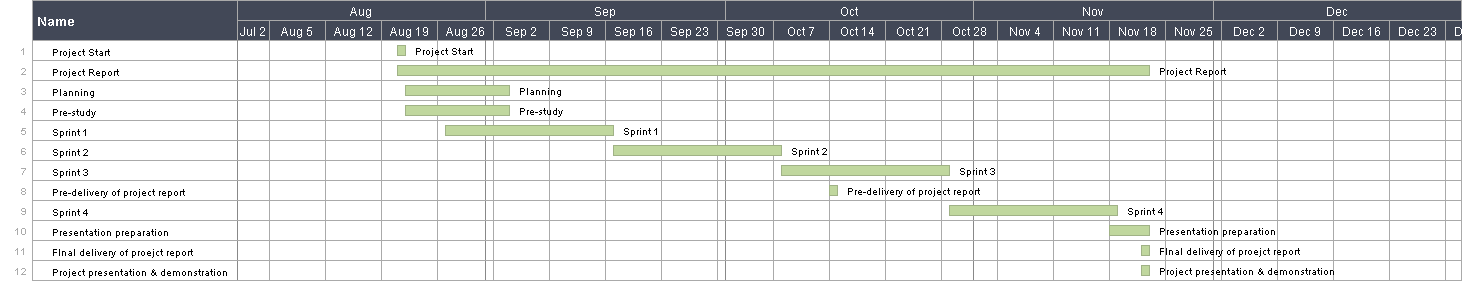
\includegraphics[width=\textwidth, height=2.5in]{foo}
\caption{Gantt-diagram for the entire project}
\end{center}
\end{figure}

%\chapter{Planning}

	\include*{measurement_of_project_effects}

	\include*{limitations}

	\include*{tool_selection}

	\include*{concrete_project_work_plan}

	\include*{sprint-summary}

	\include*{wbs}

\newpage	

	\include*{project_organization}	

	\include*{quality_assurance}

\newpage

	\include*{templates_and_standards}

	\include*{version_control_procedures}

	\include*{design_guidelines}

	\include*{table_for_handling_of_risks}

	\LTXtable{\textwidth}{risktable.tex}
	
%\chapter{Requirements}

	%

\chapter{Requirements}

\section{Business requirements}

\subsection{Quality requirements}

\subsubsection{Functional requirements}
See table \ref{tab:functionalreq} at page \pageref{tab:functionalreq}.

\begin{table}
\begin{tabular}{p{1.5cm}|p{12.5cm}|p{2cm}}
\textbf{Req.} & \textbf{Description} & \textbf{Priority} \\ \hline \hline
\textbf{FR1} & \textbf{Starting application and logging in:}The user has to be able to start the application and authorize himself against an authorizing mechanism. & High \\ \hline
\textbf{FR2} & \textbf{Send a message to another user:}The user has to be able send a simple message via regular email protocols to a recipient of own choice. & High \\ \hline
\textbf{FR3} & \textbf{Browse received messages:} The user has to be able to browse all messages he has received. & High \\ \hline
\textbf{FR4} & \textbf{Browse sent messages:} The user has to be able to browse all messages he has sent, and see the status of a sent message, where the relevant statuses are “message delivered” and “message read”. & High \\ \hline
\textbf{FR5} & \textbf{Viewing address book:} The user has to be able to view the address book with all contacts, so that he is able to choose a recipient from a list when he wants to send a message. & High \\ \hline
\textbf{FR6} & \textbf{Marking messages with a grade of importance:}The user has to be able to set Security Label, Message Priority and Message Type on a message, so that the receiver of the message knows who the message is intended for, how important it is and in what environment it is is of interest. The Message Priority will decide how intrusive XOXOmail is, that is, how much ihe app takes over the phone in order to show the user that a message has arrived.  & High \\ \hline
\textbf{FR7} & \textbf{Sending and receiving message with attachments:}The user has to be able to add an attachment to the message, so that the recipient gets the attachment as well as the message. By opening the message, the attachments will also show. & Medium \\ \hline
\textbf{FR8} & \textbf{Answer, delete and forward messages:}The user has to be able to, by clicking on a message, choose if he wants to answer, delete or forward the message, and be brought to the correct screen for doing the selected action. & Medium \\ \hline
\textbf{FR9} & \textbf{Send instant message:}The user has to be able to, via very few screen interactions, send an instant message with a predefined security label and priority, to a predefined list of recipients. & Medium \\ \hline
\textbf{FR10} & \textbf{Settings menu:}The user has to be able to alter the following settings: 
\begin{itemize}
\item{}Change default values of dropdown menus in the New Message window.
\item{}What the lowest security priority is before the message is sent via SMS
\item{}Setting text size in GUI, e.g. on received message text.
\end{itemize}  & Low
\end{tabular}
\caption{Functional requirements} \label{tab:functionalreq}
\end{table}

\subsubsection{Quality requirements}

\paragraph{Usability}
\subparagraph{U1 Ease of use}\hfill
\newline
The user should be able to use the program with very few mistakes, such as pressing the wrong button because button labels are ambiguous or too small.
\newline
\newline
See table \ref{tab:easeofuse} at page \pageref{tab:easeofuse}.
\begin{table}
\begin{tabularx}{\linewidth}{>{\setlength\hsize{.3\hsize}}X|>{\setlength\hsize{0.7\hsize}}X}
\textbf{Portion of scenario} & \textbf{Values} \\ \hline \hline
Source & End user \\ \hline
Stimulus & Use system without problems \\ \hline
Artifact & System \\ \hline
Environment & At run time \\ \hline
Response & Provide clean and understandable interface \\ \hline
Response measure & Maximum 5\% of user operations should be mistakes (another action than the user wanted).
\end{tabularx}
\caption{Ease of use} \label{tab:easeofuse}
\end{table}

\subparagraph{U2 Efficent use}\hfill
\newline
The user should be able to use the main features of the program with as few clicks as possible. Streamlined design is therefore of great importance.
\newline
\newline
See table \ref{tab:efficentuse} at page \pageref{tab:efficentuse}.
\begin{table}
\begin{tabularx}{\linewidth}{>{\setlength\hsize{.6\hsize}}X|>{\setlength\hsize{1.4\hsize}}X}
\textbf{Portion of scenario} & \textbf{Values} \\ \hline \hline
Source & End user \\ \hline
Stimulus & Use system efficiently \\ \hline
Artifact & System \\ \hline
Environment & At run time \\ \hline
Response & Organize application so that important functions are easy to reach from the main menu. \\ \hline
Response measure & A user with only a quick (5 min) training course should never spend more than one minute finding what he looks for.
\end{tabularx}
\caption{Efficent use} \label{tab:efficentuse}
\end{table}

\newpage
\paragraph{Performance}
\hfill
\newline
See table \ref{tab:performance} at page \pageref{tab:performance}.
\begin{table}
\begin{tabularx}{\linewidth}{>{\setlength\hsize{.6\hsize}}X|>{\setlength\hsize{1.4\hsize}}X}
\textbf{Portion of scenario} & \textbf{Values} \\ \hline \hline
Source & End user \\ \hline
Stimulus & Wants to open message \\ \hline
Artifact & System \\ \hline
Environment & Under normal operations \\ \hline
Response & The operation is performed \\ \hline
Response measure & With a latency of maximum 3 seconds, the user should be able to read the message after it is received. This is the latency when we subtract the download time of message, which is dependent of the network connection.
\end{tabularx}
\caption{P1 Latency} \label{tab:performance}
\end{table}

\paragraph{Security}
\hfill
\newline
See table \ref{tab:s1}, \ref{tab:s2} and \ref{tab:s3} at pages \pageref{tab:s1}, \pageref{tab:s2} and \pageref{tab:s3}.
\begin{table}
\begin{tabularx}{\linewidth}{>{\setlength\hsize{.6\hsize}}X|>{\setlength\hsize{1.4\hsize}}X}
\textbf{Portion of scenario} & \textbf{Values} \\ \hline \hline
Source & Unauthorized user or app \\ \hline
Stimulus & Wants to access data saved by our app \\ \hline
Artifact & System \\ \hline
Environment & Under normal operations \\ \hline
Response & User is blocked from accessing data by the Android OS, as long as the user doesn’t have root access. \\ \hline
Response measure & No data exposed to the user or app, as long as the user do not have root access.
\end{tabularx}
\caption{S1 Accessing locally stored data outside of app} \label{tab:s1}
\end{table}


\begin{table}
\begin{tabularx}{\linewidth}{>{\setlength\hsize{.6\hsize}}X|>{\setlength\hsize{1.4\hsize}}X}
\textbf{Portion of scenario} & \textbf{Values} \\ \hline \hline
Source & Unauthorized user \\ \hline
Stimulus & Wants to use app features \\ \hline
Artifact & System \\ \hline
Environment & Under normal operations \\ \hline
Response & User is blocked from using functions \\ \hline
Response measure & No features exposed to the user - stopped by login screen
\end{tabularx}
\caption{S2 Trying to use app with wrong privileges} \label{tab:s2}
\end{table}

\begin{table}
\begin{tabularx}{\linewidth}{>{\setlength\hsize{.6\hsize}}X|>{\setlength\hsize{1.4\hsize}}X}
\textbf{Portion of scenario} & \textbf{Values} \\ \hline \hline
Source & Unauthorized user or app, or someone sniffing network packages \\ \hline
Stimulus & Wants to access data stream \\ \hline
Artifact & System \\ \hline
Environment & Under normal operations \\ \hline
Response & Is unable to get useful information because of SSL encryption \\ \hline
Response measure & No useful data exposed to the user
\end{tabularx}
\caption{S3 Trying to access the apps external data traffic} \label{tab:s3}
\end{table}

\subsubsection{Component and Technology related constraints}
Vanilla Android is the platform of choice, compatible down to Android API 8

\paragraph{Programming language} \hfill
\newline
Developing for Android will in this project mean that code will be written in Java for the Dalvik Virtual Machine. This means that there is no support for multiple inheritance, and this limits design choices to some degree. It prevents us from playing with some more complicated architectures and inheritance schemes.

\paragraph{Mobile devices} \hfill
\newline
Android is a mobile OS, so the program will run on cell phones and potentially tablets. 

\paragraph{Input methods} \hfill
\newline
Android phones have small screens and usually no keyboard. This means that the user interface must be designed to work with small touch screens as the only input method.

\paragraph{Memory}\hfill
\newline
Phones have limited memory, typically 256-512 MB. The program will probably never be close to breaking this limit, as the most memory consuming components are string based e-mails and potentially an attachment or two; very little of which has to remain in memory at the same time.

\paragraph{Screen resolution/aspect ratio} \hfill
\newline
As the program will support different Android devices, it also has to support different resolutions as well as aspect ratios. The GUI must be programmed to scale to different formats without degrading quality or proportions.

\paragraph{Bandwidth} \hfill
\newline
Since the program is network based, it is important to pay attention to bandwidth usage. We want to be able to wait for incoming emails and receive them as soon as the server does without having to waste bandwidth with constant probing, especially as the program is expected to see some use outside of 3G net areas.

\paragraph{Commercial off-the-shelf (COTS)} \hfill
\newline
This project has security requirements that require special consideration with regards to COTS. We have to be able to trust the underlying software if it ever touches unencrypted data or has access to a memory partition (either legitimately or not) that contains unencrypted data. This means some care has to be taken in regards to what COTS solutions we can use and where we can use them. 

\subsubsection{Stakeholders and their concerns}
See table \ref{tab:stakeholders} at page \pageref{tab:stakeholders}.

\begin{table}
\begin{tabular}{p{3.5cm}|p{11.5cm}}
\textbf{Stakeholder:} & \textbf{Concern} \\ \hline \hline
User & 
\begin{itemize}
\item{} Wants a program that works out of the box
\item{} Easy to understand the flow of the app
\item{} Installation should be easy, just download the app from   Android market, and it’s ready to use.
\item{} Familiar user interface
\end{itemize}\\ \hline
Developers & 
\begin{itemize}
\item{}Easy to understand the goal of the app
\item{}Easy to extend and change the app
\item{}Want to use technology they are familiar with
\item{}Easy to understand Requirements and Architectural description documents.
\end{itemize}\\ \hline
Android market & 
\begin{itemize}
\item{}Make sure our game complies with regulations for software being sold/provided on Android Market.
\end{itemize}\\ \hline
Course advisor & 
\begin{itemize}
\item{}Effective and healthy communication with the group.
\item{}Easy to read documentation
\item{}Gets all deliveries on schedule
\end{itemize}\\ \hline
Customer & 
\begin{itemize}
\item{}Effective and healthy communication with the group.
\item{}A working prototype that gives a possible solution to the requirements.
\item{}Wants to see what is possible on the Android platform.
\item{}Understandable Requirements and Architectural description documents.
\end{itemize}\\ \hline
Graphic designers & 
\begin{itemize}
\item{}Understanding of how the GUI should be.
\item{}Understand the limitation of graphics due to screen size.
\end{itemize}
\end{tabular}
\caption{Stakeholders and their concerns} \label{tab:stakeholders}
\end{table}

	\include*{functional_requirements}

	\LTXtable{\textwidth}{reqlongtable.tex}

	\include*{non_functional_requirements}

	\section{Use Cases}

\subsection{Actors}
An actor specifies a role that are to be played by an external person interacting with our application. We have only one actor, and that is the regular user:  A person who don’t have much education in using our app, but who will use it regularly in his workday.

\subsection{Use case diagrams}
See figure \ref{fig:usecase} at page \pageref{fig:usecase}.

\begin{figure}
\begin{center}
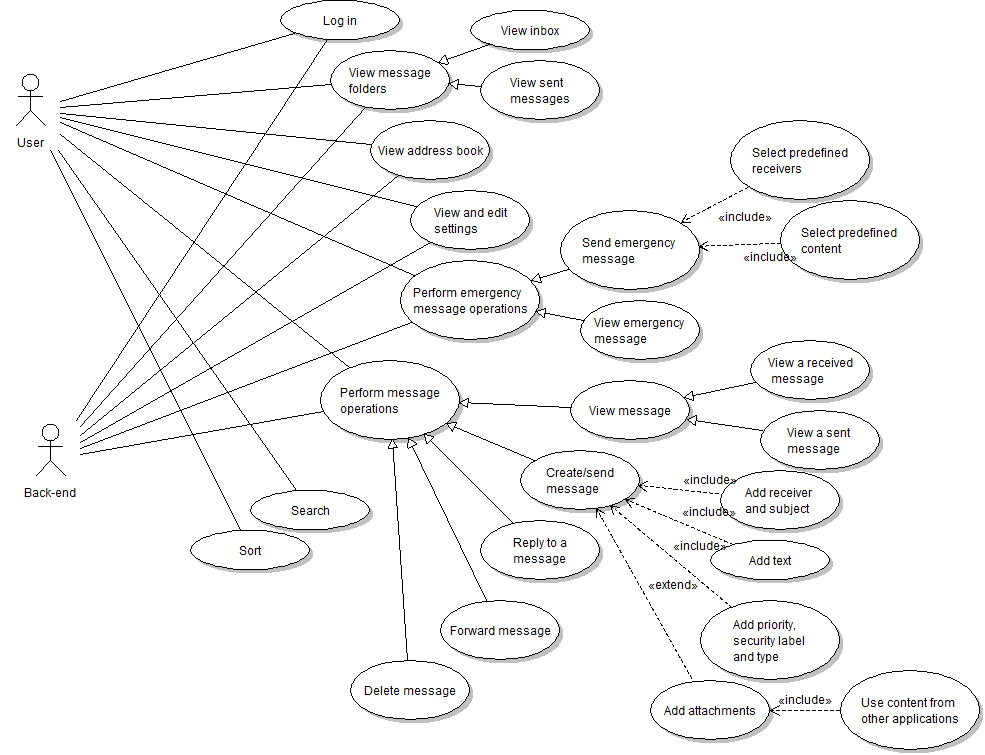
\includegraphics[width=\textwidth]{kpro-use-case}
\caption{Use case diagram} \label{fig:usecase}
\end{center}
\end{figure}

\subsection{Textual use cases}
Each of the use cases is described below, so that the use case diagram will be easier to understand. See table \ref{tab:viewmessages} - \ref{tab:settings} starting at page \pageref{tab:viewmessages} for a more detailed explanation of the use cases.


\begin{table}
\begin{tabular}{p{3cm}p{12cm}}
& 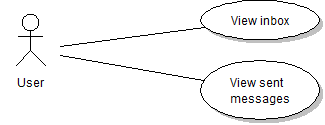
\includegraphics{view_messages}\\ \hline
Element & Description \\ \hline
Use case name & View messages \\
Goal & View received and sent messages \\
Summary &The user would like to view received and sent messages \\
Preconditions &
\begin{enumerate}
\item{}The application is running.
\item{}The user is logged in.
\end{enumerate} \\ \hline
Flow of Events &
\begin{enumerate}
\item{}The user selects a message from either the inbox or sent messages.
\item{}Message is showed to user.
\end{enumerate} \\ \hline
Exceptions & There are no existing messages.
\end{tabular}
\caption{View messages textual use case} \label{tab:viewmessages}
\end{table}

\begin{table}
\begin{tabular}{p{3cm}p{12cm}}

Element & Description \\ \hline
Use case name & Reply, forward and delete \\
Goal & Reply, forward and delete messages\\
Summary & The user would like to reply to a message, forward it or delete it. \\
Preconditions &
\begin{enumerate}
\item{}The application is running.
\item{}The user is logged in.
\end{enumerate} \\ \hline
Flow of Events &
\begin{enumerate}
\item{}The user selects a message from either the sent or inbox messages.
\item{}Message is showed to user.
\item{}User chooses to reply, forward or delete the message. 
\end{enumerate} \\ \hline
Exceptions & There are no existing messages.
\end{tabular}
\caption{Reply, forward and delete textual use case} \label{tab:viewmessages}
\end{table}

\begin{table}
\begin{tabular}{p{3cm}p{12cm}}

Element & Description \\ \hline
Use case name & View message folders \\
Goal & View inbox and sent messages \\
Summary &The user would like to view the inbox and a list of sent messages \\
Preconditions &
\begin{enumerate}
\item{}The application is running.
\item{}The user is logged in.
\end{enumerate} \\ \hline
Flow of Events &
\begin{enumerate}
\item{}The user enters the inbox or sent messages.
\item{}The list of messages in the inbox or sent messages is presented to the user.
\end{enumerate} \\ \hline
Exceptions & There are no existing messages.
\end{tabular}
\caption{View message folders use case} \label{tab:viewmessages}
\end{table}

\begin{table}
\begin{tabular}{p{3cm}p{12cm}}
& 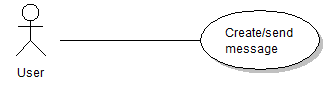
\includegraphics{create_message}\\ \hline
Element & Description \\ \hline
Use case name & Create message \\
Goal & User creates and sends a complete message \\
Summary &The user would like to create/send a message to a receiver with a subject and text. The user would also like to set the priority, security label and type of the message as well as being able to add an attachment from other applications. \\
Preconditions &
\begin{enumerate}
\item{}The application is running.
\item{}The user is logged in.
\end{enumerate} \\ \hline
Flow of Events &
\begin{enumerate}
\item{}User selects new message.
\item{}The user adds the recipient(s) and subject to the message.
\item{}The user sets the priority, security label and type.
\item{}The user adds attachments if needed.
\end{enumerate} \\ \hline
Exceptions & The user does not set priority, security label and type and default values are set.
\end{tabular}
\caption{Create message textual use case} \label{tab:createmessage}
\end{table}

\begin{table}
\begin{tabular}{p{3cm}p{12cm}}

Element & Description \\ \hline
Use case name & Send emergency message \\
Goal & User sends an emergency message \\
Summary & The user sends an emergency message with predefined content to predefined receivers \\
Preconditions &
\begin{enumerate}
\item{}The application is running.
\item{}The user is logged in.
\end{enumerate} \\ \hline
Flow of Events &
\begin{enumerate}
\item{}User selects new emergency message.
\item{}The user sends the message.
\end{enumerate} \\ \hline
Exceptions & The predefined values have not been set.
\end{tabular}
\caption{Send emergency message textual use case} \label{tab:createmessage}
\end{table}




\begin{table}
\begin{tabular}{p{3cm}p{12cm}}

Element & Description \\ \hline
Use case name & View emergency message \\
Goal & User views an emergency message \\
Summary & The user receives and viesw an emergency message \\
Preconditions &
\begin{enumerate}
\item{}The application is running.
\item{}The user is logged in.
\end{enumerate} \\ \hline
Flow of Events &
\begin{enumerate}
\item{}User receives an emergency message.
\item{}A popup appear on the users screen.
\item{}User presses the popup and views the emergency message.
\end{enumerate} \\ \hline
\end{tabular}
\caption{View emergency message textual use case} \label{tab:createmessage}
\end{table}

\begin{table}
\begin{tabular}{p{3cm}p{12cm}}
& 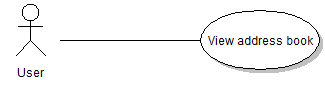
\includegraphics{view_address_book}\\ \hline
Element & Description \\ \hline
Use case name & View and interact with address book \\
Goal & User can view and interact with the address book \\
Summary &The user enters the address book and is able to view, add, edit and delete contacts. \\
Preconditions &
\begin{enumerate}
\item{}The application is running.
\item{}The user is logged in.
\end{enumerate} \\ \hline
Flow of Events &
\begin{enumerate}
\item{}User selects address book.
\item{}User either adds a new contact or selects an existing one.
\item{}If the user selects an existing contact, he can either edit that contact or delete it.
\end{enumerate}
\end{tabular}
\caption{View and interact textual use case} \label{tab:viewandinteract}
\end{table}

\begin{table}
\begin{tabular}{p{3cm}p{12cm}}
& 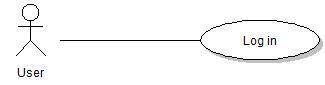
\includegraphics{login}\\ \hline
Element & Description \\ \hline
Use case name & Log in \\
Goal & User logs in with a username and password. \\
Summary &The user is prompted with a login screen and must type in his username and password. \\
Preconditions &
\begin{enumerate}
\item{}The application is running.
\end{enumerate} \\ \hline
Flow of Events &
\begin{enumerate}
\item{}User starts application.
\item{}User is prompted with username and password.
\item{}User types in username and password and presses the login button.
\item{}User gains access to the application data and functionality.
\end{enumerate} \\ \hline
Exceptions & User types wrong username and password and is denied access.
\end{tabular}
\caption{Log in textual use case} \label{tab:login}
\end{table}

\begin{table}
\begin{tabular}{p{3cm}p{12cm}}
& 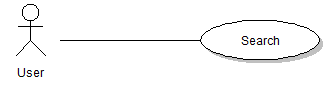
\includegraphics{search}\\ \hline
Element & Description \\ \hline
Use case name & Search \\
Goal & User receives search results for a given search text. \\
Summary & The user search in the application for mail, contacts etc through a search field at the top of the screen. \\
Preconditions &
\begin{enumerate}
\item{}The application is running.
\item{}The user is logged in.
\end{enumerate} \\ \hline
Flow of Events &
\begin{enumerate}
\item{}User highlights search field and inserts his the text he wants to search for.
\item{}User presses the search button.
\item{}Application shows search results to the user.
\end{enumerate}
\end{tabular}
\caption{Search textual use case} \label{tab:search}
\end{table}

\begin{table}
\begin{tabular}{p{3cm}p{12cm}}
& 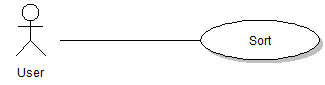
\includegraphics{sort}\\ \hline
Element & Description \\ \hline
Use case name & Sort \\
Goal & User sorts the messages in his inbox. \\
Summary & The user chosoes a value that he wishes the messages to be sorted by. \\
Preconditions &
\begin{enumerate}
\item{}The application is running.
\item{}The user is logged in.
\item{}There are messages to sort.
\end{enumerate} \\ \hline
Flow of Events &
\begin{enumerate}
\item{}The user selects the value he wishes the messages to be sorted by.
\item{}The application sorts the messages and displays them to the user.
\end{enumerate}
\end{tabular}
\caption{Sort textual use case} \label{tab:search}
\end{table}

\begin{table}
\begin{tabular}{p{3cm}p{12cm}}
& 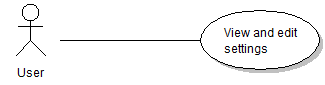
\includegraphics{settings}\\ \hline
Element & Description \\ \hline
Use case name & Settings \\
Goal & The user can alter settings. \\
Summary & The user enters the settings menu and alter the settings to suit his own preferences. \\
Preconditions &
\begin{enumerate}
\item{}The application is running.
\item{}The user is logged in.
\end{enumerate} \\ \hline
Flow of Events &
\begin{enumerate}
\item{}User presses the settings button.
\item{}User alters the settings he wishes to.
\item{}Application saves the alterations.
\end{enumerate}
\end{tabular}
\caption{Settings textual use case} \label{tab:settings}
\end{table}


	%\section{User Stories}

	\include*{requirements_from_customer}

%\chapter{Project study}

	\chapter{Project study}

This Chapter will cover the preliminary studies carried out in this project and will provide an understanding of what the problem to be solved, what solutions exist already and what solutions we have chosen.

\section{Problem description}

\subsection{Thales}
Thales wants us to develop a message service that is custom made for mobile users, with a user-interface that has good affordance and is easy and effective to use.
\newline
\newline
The users of this application are people who need a reliable and secure way of communicating with more or less time dependent information. Users are also expected to only have access to either tablets or mobile phones, not computers.

\subsection{Functionality}
The application's functionality should be similar to a normal email client, but with a user-interface that is custom-made for smaller screens, short messages, military domain specific  attributes, reliability adjustments for field use and security adjustments for handling classified information. The application should use the Simple Mail Transfer Protocol to communicate with Thales' XOmail \gls{smtp} gateway.
\newline
\newline
The application should not use bandwidth when it is not sending or receiving messages. The application should also be able to receive an updated address book from the server.

\subsection{The solution}
As per the customer requirements, the solution is to be implemented on Android based smartphones or tablets (Requirement 1.1 and 1.2) and the user-interface should be fitted to the screen size of the given device (2.1). It should support bandwidths as small as 64 kbps (2.2) and communicate with a XOmail server through \gls{pami}/\gls{pop} and \gls{smtp}(1.4 and 2.3). The application should also work with normal mail servers, but with reduced functionality (2.4).
\newline
\newline
The messages sent with our solution should be able to support text, pictures and video attachments (3.1). The media should be accessed from the local storage on the phone or from other applications (3.2). A user should be able to create, edit, send, answer, forward and delete messages as well as browse and open received and sent messages (3.3)

\subsection{Military attributes}
The messages that a user sends should support certain military attributes, these include precedence, type and security label. Precedence is an indicator that indicates the level of urgancy, and type indicates the type of the message. Security label on the other hand says something about the reciever of the massage, and not the massage itself. The security label says what security clearance the receiver must have to be able to open the message.
\newline
\newline
One should also be able to ask for a delivery report and a receipt notification from the recipient of the message sent. The one who sends the message should be able to see the status on the delivery report and receipt notification.

\subsection{Instant messages}
Another message functionality is the ability to send instant messages with predefined military attributes to a predefined reciever. The reciever can be a group or a single reciever. These can include predefined text or information from another application. It should also be possible to send messages with content that is created by other applications on the device.
\newline
\newline
When a message that is sent from the application fails, the user should get a notification and the message should be sent again automatically. These messages should also be sorted by priority.

\subsection{High priority messages}
If a high priority message arrives on a given user’s phone, the application should alert the user in a convenient way and make it easy to access the newly arrived message. The application should stop the sending of all other messages when a user sends a message with high priority, and instead give the resources to the high priority message.  

\subsection{Security}
Security is also an important issue in the application. Communication with the server should be encrypted with \gls{ssl1}, messages should be signed with \gls{emims} when being sent, \gls{emims} signed messages should be verified on receive and private keys for
signing mail should not be stored in cleartext.


	\section{Current system}\label{sec:currsys}

At the moment, there are no mobile solutions to the already existing XOmail system on computers.

\subsection{XOmail - Secure message based information handling}

XOmail is a message system tailored for messaging within military organizations. The messaging functions within the system are suited for the needs of large organizations with the ability to differentiate between social messages to the entire organization and personal messages to individual users. XOmail has the ability to send messages to predefined  distribution lists where the messages gets distributed based on a given criteria like the subject of the message. 
\cite{bib:XOhome}
\newline
\newline
The system also has several APIs that can be accessed by other applications. XOmail supports message coordination for use in the drafting process, as well as the ability to have a release authority for a drafted message. Another feature of XOmail is the ability to add precedence to messages, giving high priority messages access to resources and communication channels before messages with lower precedence. This is very important in a military setting. 
\cite{bib:XOhome}
\newline
\newline
XOmail has also a high focus on security, and offers security for the messaging platform, servers and gateways. The system also has an extensive administration tool that can be accessed both locally and remotely.
\cite{bib:XOhome}
\newline
\newline

\begin{figure}[h!]
\begin{center}
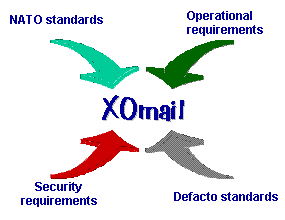
\includegraphics{xomaillogo}
\end{center}
\caption{XOmail logo} \label{fig:xomail}
\end{figure}

	\include*{planned_solution}

	\include*{similar_solutions}

	\include*{waterfall_vs_agile}

	\include*{programming_languages}

	\include*{markup_languages}

	\include*{parsers_libraries_and_tools}

\newpage

	\include*{unit_testing_frameworks}

	\include*{user_documentation_tools}

	\include*{integrated_development_environment}

	\include*{remote_vs_local_service}

	%\section{Secure storage}
In the application we are developing we need some way of authenticating users and granting them access to the features of the application. We want the users to log in using a username and password and also allowing them to save the password so that the user does not have to retype the password every time they open the application. This feature introduces many security issues. 

\subsection{Local storage with username and password}
One solution is to store the username and password locally on the phone. In Android applications this is usually done in SharedPreferences. SharedPreferences is sandboxed and thus preventing other applications from accessing the values stored there. If you also encrypt the credentials instead of just storing them as plaintext it would add even more security. 
\newline
\newline
The problem with this solution is if an attacker should in some way gain physical access to your phone. If you are already logged in, the perpetrator could just open up the application and view the data he wants. Even if you weren’t logged in the attacker could root the phone and gain access to the values saved in SharedPreferences. Even if the values are encrypted it would not help, because an attacker that has access to the values in SharedPreferences is also likely to have access to the applications binary, and thus the keys to decrypt the password.

\subsection{Creating a custom account type}
Another solution is to create an online user account and add this to the centralized AccountManager registry. The user can then type in his username and password once, and gain access to the various resources online. The credentials are here authenticated on the server and we can therefore store the credentials as a cryptographically secure token on the device. This would make sure that an attacker would not get access to your actual username and password. 
\newline
\newline
This solution also suffers from the fact that if the user is already logged in, the attacker could view all the information. One could solve this by implementing a timeout on the application (If the user does not perform an action after x minutes, the application is terminated and the user gets disconnected).

\subsection{Symmetric encryption}
Symmetric encryption is also a possible solution. If you are going to use this type of encryption you can’t store the keys because of the lacking general purpose, system-level secure storage. A way to solve this is to derive the keys from a user-entered password. To make sure the keys derived are random and hard to brute-force we need to use a standard \gls{pbe} key derivation method. For android applications this is called PBKDF2WithHmacSHA1.
\newline
\newline
This could be a suitable solution, at least for the parts of the application that does not need to happen instantantly. 


	\include*{security_requirements}

	\include*{secure_communication}

	\include*{secure_storage}

	\include*{wireshark}

\newpage

	\include*{compression_of_data}

	\include*{ip_rights_and_licenses}

	\include*{evaluation_criteria}


%\chapter{Test plan}

	\chapter{Test plan}

This chapter will describe how we plan to test the application, both continuously and at the end of the project. Section 6.1 describes what methods we plan to use to test our code. Section 6.2 describes the different test tools we will use in the project and why these were used. Section 6.3 details the design verification to be carried out. Section 6.4 details the plan for testing functionality and usability of the project. 

\section{Methods and goals for testing}

The main part of project testing will be done as we go along. Using unit tests, each part of the code will be thoroughly tested before it is put together. Larger scale integration and instrumentation tests are done largely the same way, compounded by informal testing by group members. The sending and receiving of messages will be tested using Greenmail, while Mockito is used to handle not yet implemented classes as well as emulator free testing for Android specific classes. All of these tools are described in the section below. Towards the end of the project period, including large parts of the fourth sprint, the focus will shift from producing additional code to finding and repairing bugs. While our plan is vaguely based upon, and in large part inspired by, \gls{ieee829} \cite{bib:ieee} we are too informal about it to be able to use such grand claims. In short, our testing plan is to test each public method both for valid and invalid input, and then run larger scale integration tests between modules.
By using dependency injection and Mockito, we will also be able to test top level modules without testing the building blocks of that module. 
\newline
\newline
The overall goal for the test plan is that every part of our code related to the backend service is tested thoroughly, both for valid and invalid input. Though the same would be good for the frontend,
it is harder to do this automaticly, and therefore it will only be tested whether or the functionality works or not. The optimal goal would be 100\% code coverage, but this is rarely feasible, hence
we will settle for anything between 60-80\%. 
\newline
\newline
In order to ensure the greatest possibility of correctness for our code, each member of the team will be responsible for writing test for their code before it is submitted to our common repository.
Changes in the user interface should also be tested, though if there is no automatic way of doing it, one should tests all functionality related to the changes one have made in the code. 



\section{Test tools}
This section will describe the different test tools we plan to use and sums up with why these tools were selected.
\subsubsection{JUnit}
JUnit is the industry standard for test driven development. It works by creating a separate test method for each method in the class that is to be tested. In this way one can test large portions of code independent of the other code sections. For us, it provides many benefits, especially that most of us have dealt with it before and are familiar with the concept.

\subsection{Cobertura}
Cobertura is a tool for calculating the code covered by our tests, and generate a report based on this. While all other testing tools are automatically run at each build cycle, this is not the case with
Cobertura, which need to be invoked by a seperate command. 

\subsection{Mockito}
Mockito is a simple and elegant \gls{api} for mocking classes. With a few lines of code an unimplemented class can be instructed to provide a valid output, allowing other parts of the code to be tested without concerns.

\subsection{Greenmail}
Greenmail is an open source mail server package for testing in Java. It provides all the server side software needed to test simple sending and receiving of mail without having an actual server. 
It does, however, not support the \gls{pami} IDLE, which in turn forced us to test this feature manually.


\subsection{Why we selected these test tools}
The choice of tools was mainly based on previous experience inside the group, the framework provided by and the demands of the platform. 
\newline
\newline
\gls{junit} was chosen because of our previous experience and the fact that the Android instrumentation framework is based on \gls{junit}. Bundled with Mockito it also gives us the possibility to test otherwise Android dependent modules in a Java environment with the Android specifics mocked up. This can greatly reduce the build cycle time, since the tests no longer need to be pushed onto a device in order to run. Mockito also provides another benefit, in that you can test a component without testing its dependencies. This allows for highly specific testing of just one class, component or module.
\newline
\newline
Greenmail was chosen based on the need to test the message module in our project, ease of use and fast response time. If the code passes the Greenmail tests, the code is then tested against gmail’s mail server to ensure that functions with external servers as well. 


\section{Design Verification}
In order to accommodate the agile development plan used by the team, our early design verification is necessarily somewhat vague. In the early stages of the project we had limited knowledge of how the final product would be structured and which features it would involve.
\newline
\newline
Early in the first sprint we decided upon a set of basic interfaces, which neatly split up the project into manageable parts. We began early by writing up tests for future classes that implemented these interfaces, allowing low level testing of individual methods. At the time of writing these tests we had no idea how each method was going to be implemented. This enabled us to write generic black box tests.
\newline
\newline
Later in the project this method level testing will be augmented by white box and stress testing; essentially us deliberately trying to crash the system with strange inputs or action combinations. 


	\include*{test_cases}

%\chapter{Architectural description}
	
	\chapter{Architectural description}
	This chapter will revolve around the final architecture of the prototype created during this project. In our definition of architecture, will have choosen to follow the definition carved out by
	Len Bass, Paul Clements and Rick Kazman. ``The software architecture of a program or computing system is the sructure of structures of the system, which comprise software elements, the externally visible properties of those elements, and the relationships between them''\cite[p. 3]{bib:archi}
	
\section{Architectural Drivers}
	From the nature of the assignment and the requirements received from the customer, we decided that Security had to be one of our quality attributes. After the first couple of meeting with the customer, it became clear that usability also was something of interest to them, and we decided to add Usability to our quality attributes as well. It should however be noted that	all of the quality attributes specified in Len Bass's book 'Software Architecture in Practice'\cite{bib:archi} had their place within this project. Especially Modifiability was one of those that, though not of out main attributes, was given a fairly large amout of consideration in order to ease development at later stages of the project. The reason as to why Modifiability was not one of our main attributes comes down to the expected lifespan of the prototype, which in this case comes down to the success of the project, and what conclusions the customer sees when presented with the final prototype and documentation. However, the project revolves around making a prototype and documenting the steps taken to complete that process, and it is therefore safe to assume that the lifespan of the prototype will be relatively short. 

\section{Architectural viewpoints}
The ``4+1 view model''� \cite{bib:vm} by Philippe Kruchten suggest four different views, logical, process, development and physical. In the case of XOXOmail we are going to use the logical, process and development view. The rationale behind removing the physical view is that XOXOmail will run on a single physical device and only utilize one process, a security view, describing the layers of security, will be added instead.

\subsection{Development view (Subsystem decomposition)}
The development view is a step up from the logical view and focuses on software modules instead of classes. These subsystems/modules are organized in a hierarchy of layers where each layer provides a well-defined interface to layers above. ``The complete development architecture can only be described when all the elements of the software have been identified. It is, however, possible to list the rules that govern the development architecture: partitioning, grouping, visibility'' \cite{bib:vm}. 
Figure \ref{fig:developmentview} at page \pageref{fig:developmentview} shows the Backend Service Connects to all parts of our app. The main focus of this view is to show that it is also the connector to the external part of the app, the SMTP Gateway. This gateway is implemented by Thales, and all we have to do is connect to it using well known protocols.

\begin{figure}[H]
	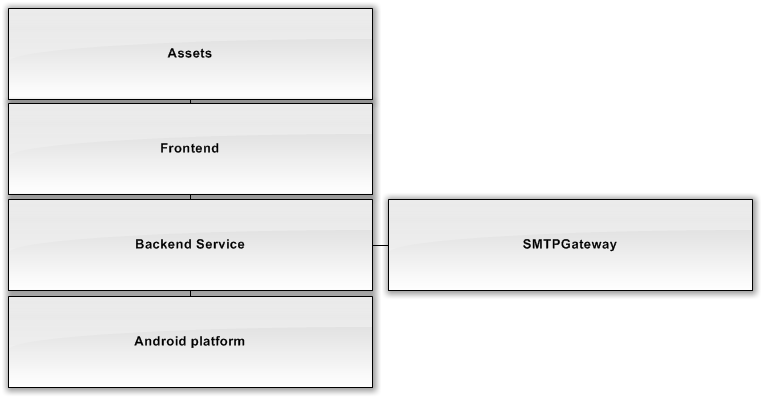
\includegraphics[width=\textwidth]{developmentview.png}
	\caption{Development View}
	\label{fig:developmentview}
\end{figure}

\subsection{Logical view (Object oriented deomposition)}
``The logical architecture primarily supports the functional requirements --- what the system should provide in terms of services to its users. The system is decomposed into a set of key abstractions, taken from the problem domain, in the form of objects or object classes''\cite{bib:vm}. A common way to represent this view is with a class diagram that shows a set of classes and their relationships, we have however used a slightly modified varient, in order to make all the figures more readable.\newline\newline
	\subsubsection{Backend}
\begin{figure}[H]
	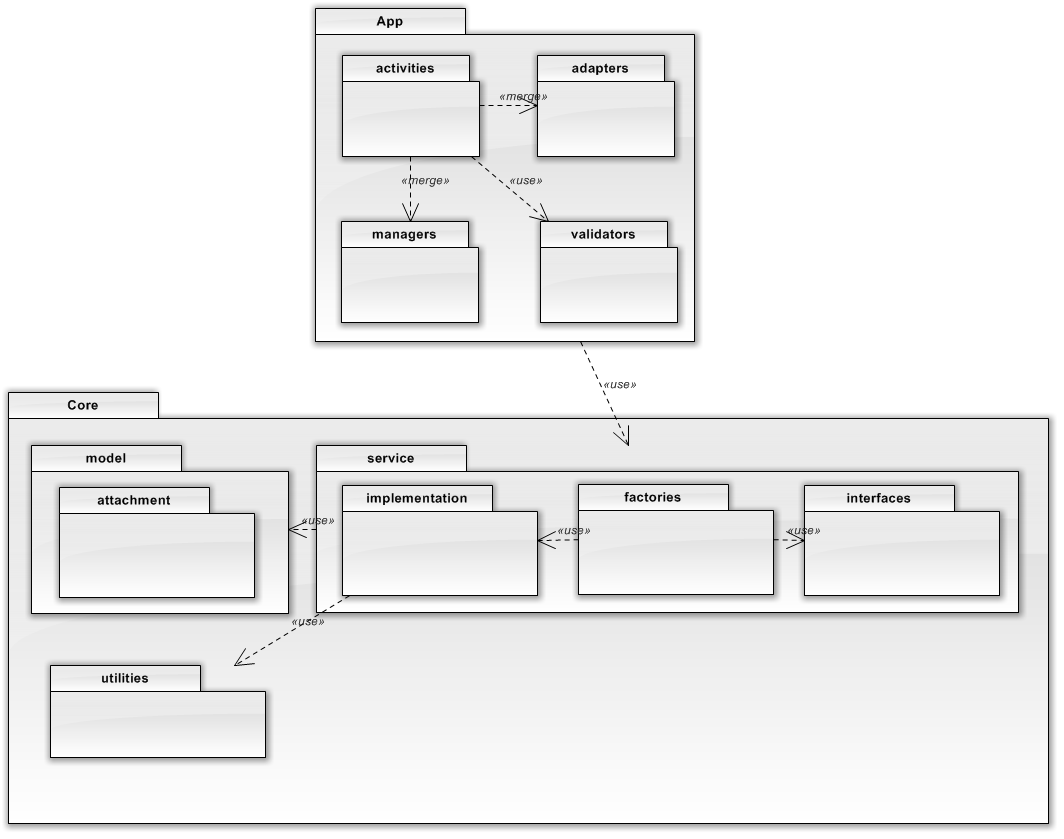
\includegraphics[width=\textwidth]{packageDiagram.png}
	\caption{The logical package view of the architecture}
	\label{fig:logicalpackview}
\end{figure}
Figure \ref{fig:logicalpackview} shown at page \pageref{fig:logicalpackview}, shows a package overview over the project backend. Though very generic, it shows the basic structure of the architecture, and the communication paths between packages. On thing to note, is that in order to add a new service to the architecture, one would need to implement three different objects, a factory for creating the service, an interface describing the service, and the service implementation itself. In the case of XOXOmail, we planned out four different services, the \textit{NetworkService}~(Fig.~\ref{fig:logicalnetworkpackview}~p.~\pageref{fig:logicalnetworkpackview}), \textit{PersistenceService}~(Fig.~\ref{fig:logicalpersistencepackview}~p.~\pageref{fig:logicalpersistencepackview}), \textit{HALService} and \textit{SecurityService}. The two latter was though never used, and their diagrams are therefore omitted here, alongside the diagram for our \textit{Utiliteis} class. The structure of our models can be seen in figure~\ref{fig:logicalmodelpackview} at page \pageref{fig:logicalmodelpackview}

\begin{figure}[H]
	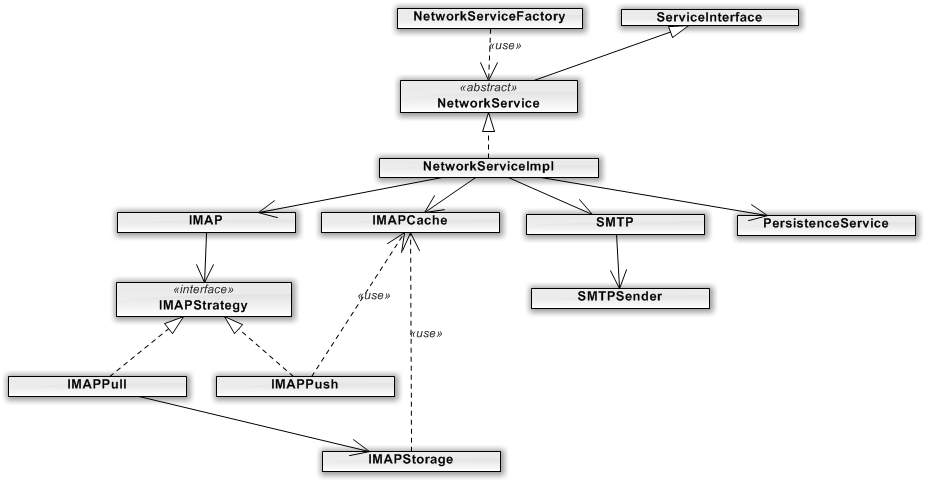
\includegraphics[width=\textwidth]{NetworkService.png}
	\caption{The logical view of the NetworkServicePackage}
	\label{fig:logicalnetworkpackview}
\end{figure}
\begin{figure}[H]
	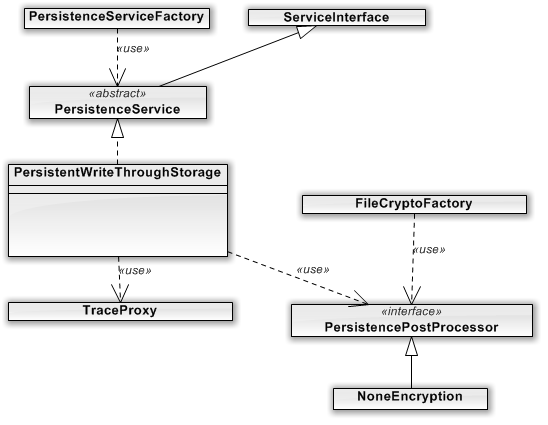
\includegraphics[width=\textwidth]{persistenceService.png}
	\caption{The logical view of the PersistenceService}
	\label{fig:logicalpersistencepackview}
\end{figure}
\begin{figure}[H]
	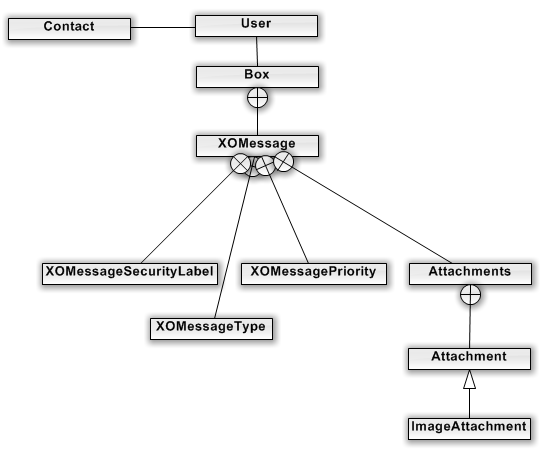
\includegraphics[width=\textwidth]{modelPackage.png}
	\caption{The logical view of the model package}
	\label{fig:logicalmodelpackview}
\end{figure}

The intended purpose of each of the different services is somewhat given by their respective names, but in order to avoid any ambiguity there will be a short recap of their purpose.
\begin{description}
	\item[NetworkService] The \textit{NetworkService}'s reponsebility is to provide the core functionality of sending and receiving mail. 
	\item[PersistenceService] The \textit{PersistenceService}'s responsebility is to keep track of objects being changes, and reflect these changes in a persistent way in case of system failure, or the application is shut down. 
\end{description}

\subsubsection{Frontend}
	\begin{figure}[H]
		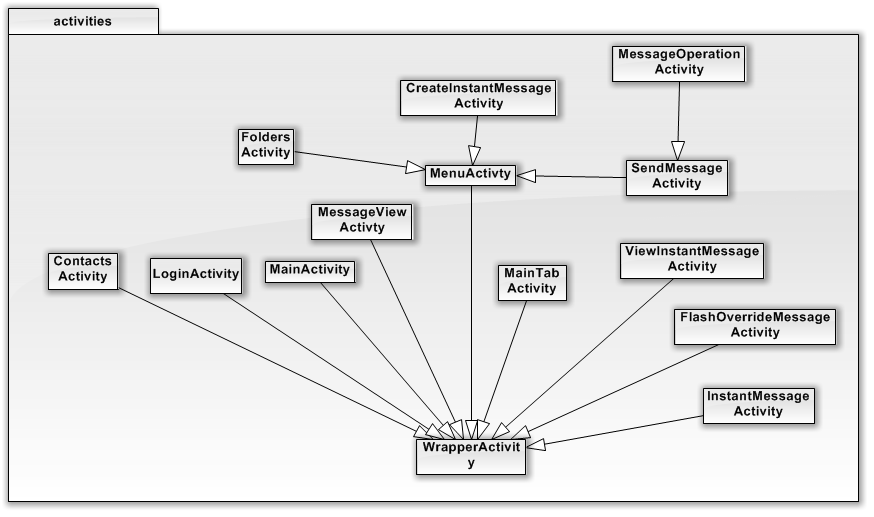
\includegraphics[width=\textwidth]{FrontendClasses.png}
		\caption{The logical view of the frontend activities package}
		\label{fig:logicalfrontpackview}
	\end{figure}	
	
\subsection{Process View}
The process view is concerned with how different tasks bind together to form one executable unit. More specifically, the communication between threads/processes and on which thread/process is a task executed. We will differentiate between major and minor tasks, where major tasks are architectural elements open through a public interface, and minor tasks being tasks introduced in order to implement some functionality in one class or module.
In figure \ref{fig:processview} at page \pageref{fig:processview}, you can differentiate between minor and major tasks by looking at the \textit{SMTP} branch of \textit{NetworkService}, here \textit{SMTPSender} is a minor task, while both \textit{SMTP} and \textit{NetworkService} is considered major tasks. 

\begin{figure}[H]
	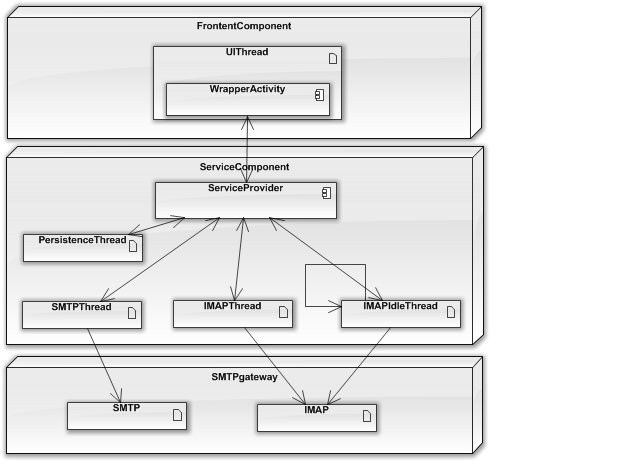
\includegraphics[width=\textwidth]{processview.png}
	\caption{Process view}
	\label{fig:processview}
\end{figure}

One thing to note about the communications paths is that all communication between the \textit{frontent component} and \textit{service component} is between two wrapper classes, \texit{WrapperActivity} at the frontend, and \textit{ServiceProvider} at the backend. 

\subsection{Security View}
The security view is concerned with how the system as a whole is secured. This involves intercommunication, storage and communication with external sources. The view is not however concerned about implementation, just the layers of security.
See figure \ref{fig:securityview} at page \pageref{fig:securityview}.

\begin{figure}[H]
	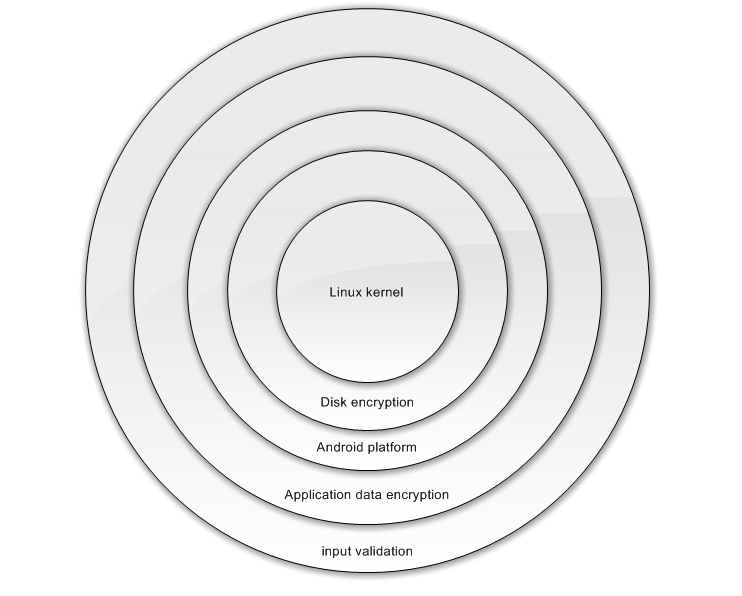
\includegraphics[width=\textwidth]{securityview.png}
	\caption{Security view}
	\label{fig:securityview}
\end{figure} \hfill
\newline
\newline
\textbf{The Linux kernel} provides us with a user-based permissions model and process isolation, which ensures that another process cannot access the memory of XOXOMail during runtime.
\newline
\newline
\textbf{Disk encryption}, is feature provided by the android platform, which encrypts the whole Android device using \gls{aes} with \gls{cbc} and \gls{essiv2}.\cite{bib:crypto}
\newline
\newline
\textbf{Android platform}, most of the security provided by the Android platform is provided by the Linux kernel, but not necessary used in normal conditions. The application sandbox is one of these things. And since the sandboxing operation is located at kernel level, it is hard to break out of. 
\newline
\newline
\textbf{Application data encryption} is a response to the possibility of rooted devices. Normally an android application will not run with root access on the device, this however is not the case on rooted devices. In which case the application and user will have full access to all applications and all application data. By adding our own encryption layer with the key stored off-device we can ensure data security even with root access to the phone\cite{bib:tech}. The encryption we opted for is an \gls{aes} based encryption with a user-password derived key by \gls{pbsha}.
Regarding communication with external resources as a mail-server, it will be done over a secure communication channel providing \gls{ssl1} or \gls{tls}. 
\newline
\newline
\textbf{Input validation} is always necessary in order to provide a secure service. All input to the XOXOMail application should be validated, this is includes received mail, user-input etc. For mail validation we are going to use \gls{emims} signing and verification provided by bouncycastle. 

\section{GUI}

\subsection{Introduction}
The Android platform specifies a certain way of organizing the application, which we have tried to follow.

\subsection{External resources}
The user interface elements, ranging from whole screens (called layouts) to the structure and look of a single list element, are defined in \gls{xml} (Extensible Markup Language) and stored external to the application. An Android project contains a folder named “res” where all external resources are placed. User interface elements are stored in a sub folder called “layouts”. Other resources, e.g. colors or images, are stored inside separate sub folders. The advantage of declaring the user interface and other resources in \gls{xml} is that it enables decoupling of the presentation of the application and the code that controls the application.
\newline
\newline
All resources must be assigned an \gls{id} if they are to be referenced in the application code. All resource \gls{id}s are defined as public constants in the project's R.class, which is a class that is automatically generated during build and contains subclasses for the types of resources where we have defined at least one resource, e.g. R.layout (for user interface elements) or R.color (for definition of colors). The resources can be referenced both inside other resources and in the application code.
\newline
\newline
We also want to use styles, which are collections of properties specifying the look of a layout or a component. It can be compared to the mindset of \gls{css}, where one separate design and content. We might also consider using a theme for our application, which is a style applied to an entire activity or application. The reason behind using styles and themes would be to ensure consistent appearance across the application. 

\subsection{Activities}
Activities are components that provide a screen that the user can interact with, and are classes written in Java. Each activity has a window where the user interface is drawn. One activity is specified as the main activity and is the start screen of the application. Each activity can start another activity to perform different actions. The activities inflate the \gls{xml} layouts to form the user interface and controls the behaviour of the elements. It is also possible to create layout elements programmatically, but we have chosen not to do this as we want the decoupling mentioned above.
\newline
\newline
An activity is always in one of four possible states \cite{bib:aas}:
\begin{itemize}
\item{}Active/running: When the activity is in the foreground of the screen
\item{}Paused: When the activity has lost focus but is still visible
\item{}Stopped: When the activity is completely obscured by another activity
\item{}If an activity is paused or stopped, it is likely that the system asks the activity to finish or just kill its process, hence drops it from memory. It then has to be restarted completely.
\end{itemize}

The life cycle of an activity can be seen in figure \ref{fig:lifecycle} at page \pageref{fig:lifecycle}.
\begin{figure}
	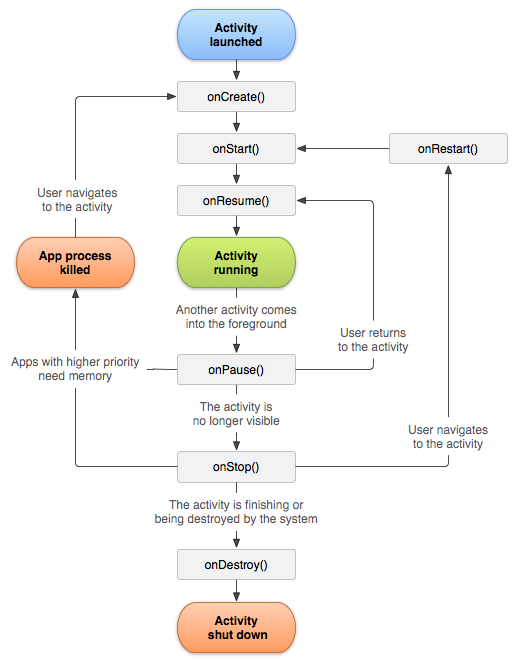
\includegraphics[width=\textwidth]{activity_lifecycle}
	\caption{Activity life cycle \cite{bib:alc}}
	\label{fig:lifecycle}
\end{figure}

All the methods starting with on (onCreate etc.) can be overwritten to administrate what the application should do in the changes of state.

\paragraph{How we did it in our app}

\begin{figure}
	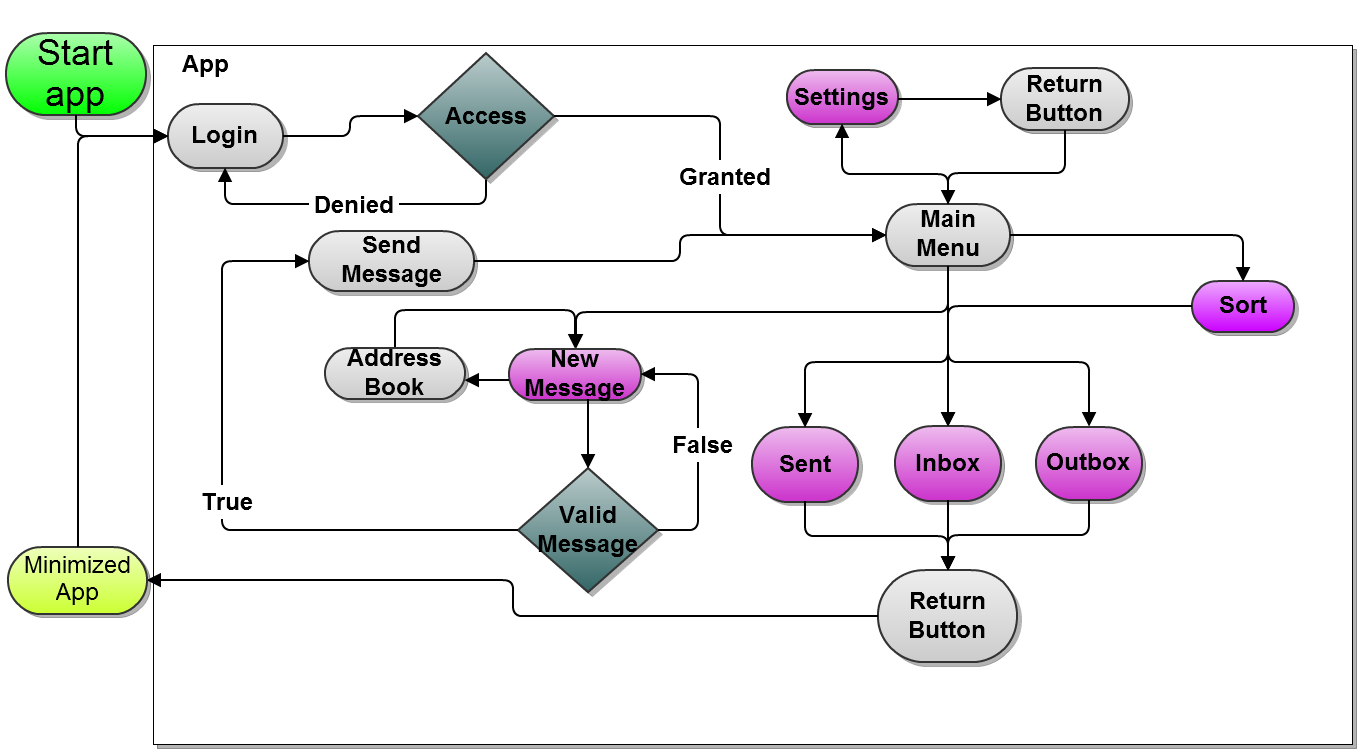
\includegraphics[width=\textwidth]{Android_GUI_flow_chart_2}
	\caption{The logical view of the GUI architecture}
	\label{fig:logicalGUIview}
\end{figure}

Figure \ref{fig:logicalGUIview} at page \pageref{fig:logicalGUIview} shows the flow in our app. It all starts in the upper left corner at "Start app". The first activity you see is the \textsc{Login Activity}. The user is granted access if a correct username and matching password is entered. He is then sent directly to the main menu, where he can choose to either see messages, send a new message or alter settings. Which messages are shown are based on if you choose \textsc{Sent}, \textsc{Outbox} or \textsc{Inbox}. By pressing \textsc{Sort} he can choose to alter the way the messages are shown. Choosing to send a message can either be done by going into the regular send message view, or the instant message view. Either way, for a message to be sent, it has to be validated. When all fields are valid, the message is sent to the correct recipient. By pressing return button when inside app we are minimizing the app. It will still be running in the background.

\subsection{The Android manifest}
The Android manifest \cite{bib:aman} is what binds the applicaiton together. It is defined in \gls{xml} and details the structure and metadata of the application, its components and requirements. The manifest needs to have nodes for each of the components, which in our case are activities and services. Relevant metadata is the application name, icon and theme. The manifest also declares the permissions the application needs to access protected parts of the \gls{api} and interact with other applications.

\subsection{Supporting different hardware and internationalization}
By conforming to using external resources on can easily build applications that support differences such as varying screen sizes and languages. For example, it is possible to create a low, medium and high dpi (dots per inch, a measure of screen density) version of an image and Android will select the correct version based on the screen size. Android can pick layouts based on the screen orientation, where the possibilities are that the phone is an portrait or landscape mode. It is also possible to have Android decide what language to use based on location, but this is not relevant to this project. 
	\include*{fulfillment_of_requirements}
	\LTXtable{\textwidth}{fulfillmentFunctionalLongTable.tex}
	\include*{fulfillment_of_requirements_rest}

\part{Scrum process}

%\chapter{Product backlog}

	\section{Product Backlog}

%\chapter{Sprint 1}

	\include*{sprint_1_planning}

	\include*{sprint_1_duration}

\newpage

	\include*{sprint_1_concrete_project_work_plan}

	\include*{sprint_1_goal}	

	\include*{sprint_1_backlog}

	\include*{sprint_1_system_design}

	\include*{sprint_1_burndown}

	\include*{sprint_1_customer_feedback}

	\include*{sprint_1_effort}
	
	\include*{sprint_1_conclusion}

%\chapter{Sprint 2}

	\include*{sprint_2_planning}

	\include*{sprint_2_duration}

\newpage

	\include*{sprint_2_concrete_project_work_plan}

	\include*{sprint_2_goal}

	\include*{sprint_2_backlog}

	\include*{sprint_2_system_design}

	\include*{sprint_2_burndown}	

	\include*{sprint_2_customer_feedback}	

	\include*{sprint_2_effort}

	\include*{sprint_2_conclusion}

%\chapter{Sprint 3}

	\include*{sprint_3_planning}

	\include*{sprint_3_duration}

	\include*{sprint_3_concrete_project_work_plan}

\newpage

	\LTXtable{\textwidth}{concrete3table.tex}

	\include*{sprint_3_goal}

	\include*{sprint_3_backlog}

\newpage

	\include*{sprint_3_system_design}

	

\newpage

	\include*{sprint_3_customer_feedback}

	\include*{sprint_3_effort}

	\include*{sprint_3_burndown}

\newpage

	\include*{sprint_3_conclusion}

%\chapter{Sprint 4}

	\include*{sprint_4_planning}

	\include*{sprint_4_duration}

	\include*{sprint_4_concrete_project_work_plan}

	\include*{sprint_4_goal}

	\include*{sprint_4_backlog}

	\include*{sprint_4_system_design}

	\include*{sprint_4_burndown}

	\include*{sprint_4_customer_feedback}

	\include*{sprint_4_effort}

	\include*{sprint_4_conclusion}

%\chapter{Changelog}
	\include*{product_backlog_changelog}

\part{Conclusion \& reflection}

	\newpage

\section{Testing}\label{con_testing}
This section will start by looking at the results from the functional testing and discuss these results, and then move on to discussing the results from the usability testing and the improvements we made from the feedback we received from the usability testing.

\subsection{Functional testing}

\paragraph{Results}\hfill
\newline
As stated in chapter \ref{chapter_test}, we tested the application continuously after implementing each functionality. However, a summary of the test results from the end of the project can be found in table \ref{tab:caseresults} on page \pageref{tab:caseresults}.
\begin{table}[h!]
\begin{center}
					\begin{tabular}{l|l|l}\hline
						\textbf{Test case ID} & \textbf{Test name} & \textbf{Result} \\ \hline \hline
						1&Login&OK\\
						2&Send regular message&OK\\
						3&Send message to contact from the address book&OK\\
						4&Send full message&OK\\
						5&Sent messages folder&OK\\
						6&Read and browse messages&OK\\
						7&Send attachments (camera)&OK\\
						8&Send attachments (gallery)&OK\\
						9&Send attachments (GPS)&OK\\
						10&Attachments received&OK\\
						11&Instant message settings&OK\\
						12&Message retrieval strategy settings&Failed\\
						13&Security labels settings&Failed\\
						14&Send instant message&OK\\
						15&Receive flash/override message&OK\\
						16&Send instant message with attachments&GPS failed, images OK\\
						17&Receive instant message outside the app&OK\\
						18&Widget for instant message&OK\\
						19&Reply&OK-\\
						20&Forward&OK-\\
						21&Delete&Failed\\
						22&Delivery report and receipt notification&Failed\\
						23&Status of delivery report and receipt notification&Failed\\
						24&Sort messages&OK\\
						25&Search in inbox&Failed\\	
						26&Login incorrect input&OK\\
						27&Receiver incorrect input&OK\\
						28&Security label incorrect input&OK\\ \hline
					\end{tabular}
\end{center}
\caption{Functional test result summary} \label{tab:caseresults}
\end{table}

\paragraph{Discussion}\hfill
\newline
The results from the final functional testing showed that 19 out of the 28 test cases passed the test,  six failed and three almost passed. Out of the six that failed, three were due to not having time to start with the implementation (test cases 22, 23 and 25) and three were known bugs that we did not get the time to fix (12, 13, 21). The three that almost passed were issues that we know how to fix but had not seen until the testing was done (16, 19, 20).


\subsection{Usability testing}
\paragraph{Results}\hfill
\newline
The results from the tests can be found in table \ref{tab:usabilitytestresults} on page \pageref{tab:usabilitytestresults}. These show that three of the goals were OK and two failed. One of the goals (4) that was not fullfilled probably happened because we did not count seconds on the tests, just whole minutes. Overall, we were happy with these results, even though we did not expect the application to crash as often as it did, as this did not happen when we tested it ourselves.

\begin{table}[h!]
\begin{center}
\begin{tabular}{l|p{6cm}|l|p{6cm}}	\hline
\textbf{Goal}&\textbf{Description}&\textbf{Status}&\textbf{Comment}\\ \hline \hline
1&The user should not spend more than 5 minutes on a task&OK&-\\ \hline
2&The application should not crash during the usability tests&Failed&The app crashed in the settings task on almost all tests\\ \hline
3&The users should not make more than 1 error during the tasks&OK&One user sent a regular message instead of an instant message\\ \hline
4&The users should solve task 6 faster than task 1&Failed&Two users spent the same amount of time, but this could also be due to the fact that the test leaders here just counted whole minutes\\ \hline
5&The average SUS score should be more than 70&OK&The average SUS score was 78.5\\ \hline 
\end{tabular}
\end{center}
\caption{Usability test - Test results} \label{tab:usabilitytestresults}
\end{table}

\subparagraph{SUS scores}\hfill
\newline
\begin{table}[h!]
\begin{center}
			\begin{tabular}{p{8cm}|l|l|l|l|l|l}	\hline
				\textbf{Question/Test}&\textbf{1}&\textbf{2}&\textbf{3}&\textbf{4}&\textbf{5}\\ \hline \hline
				1. I think that I would like to use this system frequently&3&3&4&4&3\\ \hline
				2. I found the system unnecessarily complex&2&2&2&1&2\\ \hline
				3. I thought the system was easy to use&4&4&4&5&4\\ \hline
				4. I think that I would need the support of a technical person to be able to use this system&1&2&1&1&1\\ \hline
				5. I found the various functions in this system were well integrated&3&3&3&5&5\\ \hline
				6. I thought there was too much inconsistency in this system&2&2&2&3&1\\ \hline
				7. I would imagine that most people would learn to use this system very quickly&4&3&4&4&4\\ \hline
				8. I found the system very cumbersome to use&3&2&2&1&1\\ \hline
				9. I felt very confident using the system&4&4&4&4&5\\ \hline
				10. I needed to learn a lot of things before I could get going with this system&1&2&1&1&1\\ \hline \hline
				\textbf{Score}&\textbf{72.5}&\textbf{67.5}&\textbf{77.5}&\textbf{87.5}&\textbf{87.5}\\ \hline 
				
\end{tabular}
\end{center}
\caption{Usability test - SUS scores} \label{tab:usabilitysusscore}
\end{table}
The SUS results are shown in table \ref{tab:usabilitysusscore} on page \pageref{tab:usabilitysusscore}. The average SUS score was 78.5.
\newline
\newline
			
\newpage


\begin{table}[h!]
\begin{center}
\begin{tabular}{l|l|l|l|l|l|l|l}	\hline
\textbf{Task/Time}&\textbf{1}&\textbf{2}&\textbf{3}&\textbf{4}&\textbf{5}&\textbf{Average}\\ \hline \hline
				1&1 min&1 min&1 min&1 min&1 min&\textbf{1 min}\\ \hline
				2&3 min&3 min&2 min&2 min&2 min&\textbf{2.4 min}\\ \hline
				3&3 min&4 min&4 min&5 min&5 min&\textbf{4.2 min}\\ \hline
				4&1 min&5 min&2 min&3 min&4 min&\textbf{3 min}\\ \hline
				5&1 min&1 min&0 min&2 min&3 min&\textbf{1.75 min}\\ \hline
				6&1 min&2 min&1 min&2 min&2 min&\textbf{1.6 min}\\ \hline
				\textbf{Sum}&\textbf{10 min}&\textbf{16 min}&\textbf{10 min}&\textbf{15 min}&\textbf{17 min}&\textbf{14 min}\\ \hline 
				
\end{tabular}
\end{center}
\caption{Usability test - Task times} \label{tab:usabilitytasktime}
\end{table}

\subparagraph{Time spent}\hfill
\newline
A summary of the time spent on the different tasks is shown in table \ref{tab:usabilitytasktime} on page \pageref{tab:usabilitytasktime}.
			\subparagraph{Observation forms}\hfill
\newline
The filled out observation forms can be found in appendix \ref{ch:usatest}. 

\newpage

\paragraph{Summary}\hfill
\newline
			There were many problems that reoccured in the test results. Below is a short summary of what were the problems:
			\begin{itemize}
				\item{}The testers were annoyed that the application does not remember login information
				\item{}Some were confused by odd choice of words
				\item{}The testers were annoyed that tilting of the phone sets you back to the inbox
				\item{}Almost all complained that the instant message and settings tab icons were not intuitive and spent some time finding the right tab
				\item{}Some complained about small fonts and small toasts
				\item{}Many were annoyed that the text boxes behaved weird, e.g. that the letters were not capitalized after a period and the keyboard did not always close.
				\item{}The settings were unstable and the app stopped during the task that tested the settings
				\item{}Many of the testers complained about the lack of confirmation after actions in the app
				\item{}Some testers commented that the user interface was not pretty enough
			\end{itemize}
		\paragraph{Discussion}\hfill
\newline
Even though we did not have the time to make major changes and improvements to the user interface and functionality, we learned a lot from these usability tests about how to better do things in later projects.
		
\paragraph{Redesign}\hfill
\newline
		We were able to do some minor changes in the user interface. The changes are listed below, although some of the screenshots other places may not be updated accordingly.
		\begin{itemize}
			\item{}Hopefully more intuitive icon for instant message
			\item{}Implemented bigger difference between read and unread messages in the inbox folder
			\item{}Text fields give you capitalized first letter of sentences
			\item{}Rephrased some text, e.g. "username" instead of "email" and "Take picture" instead of "Image from camera"
		\end{itemize}




%\chapter{Reflection}

	\include*{reflection}

\printglossaries
\addcontentsline{toc}{chapter}{Glossary}

\begin{thebibliography}{99}
\bibitem{bib:xomail} XOmail. Retrieved 2012-09-12 from <http://www.xomail.com>
\bibitem{bib:stanag} Stanag 4406. Retrieved 2012-09-12 from <http://www.isode.com/solutions/military-messaging.html>
\bibitem{bib:smtp} Simple Mail Transfer Protocol. Retrieved 2012-09-12 from <http://en.wikipedia.org/wiki/Smtp>
\bibitem{bib:imap} Internet Message Access Protocol. Retrieved 2012-09-12 from <http://en.wikipedia.org/wiki/Imap>
\bibitem{bib:thales} Thales Norway AS. Retrieved 2012-08-28 from <http://www.thales.no/pub/sites/index.php?siteID=4\&m=1>
\bibitem{bib:git} Git \& GitHub. Retrieved 2012-09-10 from <https://github.com/>
\bibitem{bib:android} http://developer.android.com/design/get-started/principles.html
\bibitem{bib:pandroid} http://developer.android.com/design/patterns/pure-android.html
\bibitem{bib:pke} Public Key Encryption. Retrieved 2012-09-18 from <http://en.wikipedia.org/wiki/Public\_key>
\bibitem{bib:ds} Digital signing. Retrieved 2012-09-18 from <http://en.wikipedia.org/wiki/Digital\_signature>
\bibitem{bib:smime} S/MIME. Retrieved 2012-09-18 from <http://en.wikipedia.org/wiki/S/MIME>
\bibitem{bib:gmail} Gmail and S/Mime. Retrieved 2012-09-23 from <http://www.scientificcomputing.com/is-your-e-mail-secure.aspx>
\bibitem{bib:r2mail2} R2Mail2. Retrieved 2012-09-23 from <https://play.google.com/store/apps/details?id=at.rundquadrat.android.r2mail2\&hl=no>
\bibitem{bib:waterfall} Waterfall Model. Retrieved 2012-09-23 from <en.wikipedia.org/wiki/Waterfall\_model>
\bibitem{bib:agile} Agile Development. Retrieved 2012-10-13 from <http://en.wikipedia.org/wiki/Agile\_development>
\bibitem{bib:kanban} Kanban. Retrieved 2012-10-13 from <http://en.wikipedia.org/wiki/Kanban\_(development)>
\bibitem{bib:asdas} Agile Software Development And Scrum. Retrieved 2012-09-10 from <http://www.mountaingoatsoftware.com/topics/scrum>
\bibitem{bib:scrum} Scrum (Development). Retrieved 2012-09-10 from <en.wikipedia.org/wiki/Scrum\_(development)>
\bibitem{bib:java} Java (Programming Language). Retrieved 2012-09-10 from
<http://en.wikipedia.org/wiki/Java\_programming\_language>
\bibitem{bib:andk} Android Native Development Kit (NDK). Retrieved 2012-09-10 from <http://developer.android.com/tools/sdk/ndk/index.html>
\bibitem{bib:slfa} Scripting Layer for Android (SL4A). Retrieved 2012-09-10 from <http://code.google.com/p/android-scripting/>
\bibitem{bib:php} PHP for Android (PFA). Retrieved 2012-09-10 from <http://phpforandroid.net/manual/en/index/faq>
\bibitem{bib:mbx} Monodroid by Xamarin. Retrieved 2012-09-10 from <http://xamarin.com/monoforandroid>
\bibitem{bib:xml} Extensible Markup Language (XML). Retrieved 2012-09-10 from <http://en.wikipedia.org/wiki/Xml>
\bibitem{bib:json} JavaScript Object Notation (JSON). Retrieved 2012-09-10 from <http://www.json.org/xml.html>
\bibitem{bib:xstream} Xstream. Retrieved 2012-10-27 from http://xstream.codehaus.org/
\bibitem{bib:ibm} Xstream. Retrieved 2012-10-27 from http://www.ibm.com/developerworks/java/library/x-xstream/index.html
\bibitem{bib:kolawa} Kolawa, Adam; Huizinga, Dorota (2007). Automated Defect Prevention: Best Practices in Software Management. Wiley-IEEE Computer Society Press. p. 426. ISBN 0-470-04212-5
\bibitem{bib:junit} Junit. Retrieved 2012-10-01 from http://en.wikipedia.org/wiki/JUnit
\bibitem{bib:mock} Mock objects. Retrieved 2012-10-01 from http://en.wikipedia.org/wiki/Mock\_object
\bibitem{bib:mockito} "Features and Motivations". Retrieved 2010-12-29
\bibitem{bib:mocks} Fowler, Martin (2007). "Mocks Aren't Stubs". Retrieved 2010-12-29.
\bibitem{bib:greenmail} Greenmail. Retrieved 2012-10-01 from http://www.icegreen.com/greenmail/
\bibitem{bib:latex} LaTeX. Retrieved 2012-09-25 from http://www.latex-project.org/intro.html
\bibitem{bib:atlassian} Jira overview. Retrieved 2012-09-25 from http://www.atlassian.com/software/jira/overview
\bibitem{bib:jira} Jira. Retrieved 2012-09-25 from http://en.wikipedia.org/wiki/JIRA
\bibitem{bib:green} Grennhopper. Retrieved 2012-09-25 from http://www.atlassian.com/software/greenhopper/overview
\bibitem{bib:netbeans} NetBeans. Retrieved 2012-09-25 from http://netbeans.org/features/index.html
\bibitem{bib:ide} NetBeans IDE. Retrieved 2012-09-25 from http://en.wikipedia.org/wiki/NetBeans\#NetBeans\_IDE
\bibitem{bib:service} Service. Retrieved 2012-09-08 from http://developer.android.com/reference/android/app/Service.html
\bibitem{bib:aidl} AIDL. Retrieved 2012-09-08 from http://developer.android.com/guide/components/aidl.html
\bibitem{bib:ibinder} IBinder. Retrieved 2012-09-08 from http://developer.android.com/reference/android/os/IBinder.html
\bibitem{bib:techtarget} Techtarget. Retrieved 2012-09-25 from http://searchsecurity.techtarget.com/definition/link-encryption
\bibitem{bib:ispec} IPSec. Retrieved 2012-09-25 from http://stackoverflow.com/questions/3960802/implementing-ipsec-protocol-in-java
\bibitem{bib:ssl} TLS. Retrieved 2012-09-25 from http://en.wikipedia.org/wiki/Secure\_Sockets\_Layer
\bibitem{bib:nli} NetBeans license. Retrieved 2012-10-08 from http://netbeans.org/about/legal/product-licences.html
\bibitem{bib:ali} Android license. Retrieved 2012-10-08 from http://developer.android.com/license.html
\bibitem{bib:amli} Andoid--plugin. Retrieved 2012-10-08 from http://code.google.com/p/maven-android-plugin/
\bibitem{bib:mli} Maven license. Retrieved 2012-10-08 from http://maven.apache.org/license.html
\bibitem{bib:jli} Junit license. Retrieved 2012-10-08 from http://www.junit.org/license
\bibitem{bib:gli} GreenMail license. Retrieved 2012-10-08 from http://www.icegreen.com/greenmail/
\bibitem{bib:jmli} JavaMail-android. Retrieved 2012-10-08 from http://code.google.com/p/javamail-android/
\bibitem{bib:xli} Xstream license. Retrieved 2012-10-08 from http://xstream.codehaus.org/license.html
\bibitem{bib:bcli} BouncyCastle license. Retrieved 2012-10-08 from http://www.bouncycastle.org/licence.html
\bibitem{bib:spongy} SpongyCastle, http://rtyley.github.com/spongycastle/
\bibitem{bib:lli} MiKTeX license. Retrieved 2012-10-08 from http://miktex.org/copying
\bibitem{bib:gili} Git license. Retrieved 2012-10-08 from http://git-scm.com/about/free-and-open-source
\bibitem{bib:cli} Cygwin license. Retrieved 2012-10-08 from http://cygwin.com/licensing.html
\bibitem{bib:apli} Apache 2.0 license. Retrieved 2012-10-08 from http://www.apache.org/licenses/LICENSE-2.0
\bibitem{bib:gpl1} GPL-1.0 license. Retrieved 2012-10-08 from http://www.gnu.org/licenses/gpl-1.0.html
\bibitem{bib:gpl2} GPL-2.0 license. Retrieved 2012-10-08 from http://www.gnu.org/licenses/old-licenses/gpl-2.0.html
\bibitem{bib:gplw} GPL-2.0 w/Classpath Exception license. Retrieved 2012-10-08 from http://openjdk.java.net/legal/gplv2+ce.html
\bibitem{bib:mit} MIT X11 license. Retrieved 2012-10-08 from http://opensource.org/licenses/mit-license.php
\bibitem{bib:cddl} CDDL-1.0 license. Retrieved 2012-10-08 from http://opensource.org/licenses/cddl-1.0
\bibitem{bib:cpl} CPL-1.0 license. Retrieved 2012-10-08 from http://www.junit.org/license
\bibitem{bib:bsd} BSD license. Retrieved 2012-10-08 from http://en.wikipedia.org/wiki/BSD\_licenses
\bibitem{bib:ieee} IEEE829. Retrieved  2012-09-30 from http://gerrardconsulting.com/tkb/guidelines/ieee829/main.html
\bibitem{bib:vm} Kruchten, Philippe (1995, November). Architectural Blueprints — The "4+1" View Model of Software Architecture. IEEE Software 12 (6), pp. 42-50.
\bibitem{bib:archi} Bass, Len; Clements, Paul; Kazman, Rick. Software Architecture in Practice, Second Edition.
\bibitem{bib:crypto} Android crypto implementation. Retrieved 2012-10-07 from http://source.android.com/tech/encryption/android\_crypto\_implementation.html
\bibitem{bib:tech} Security. Retrieved 2012-10-07 from http://source.android.com/tech/security/index.html
\bibitem{bib:aas} Android activity states. Retrieved 2012-10-13 from http://developer.android.com/reference/android/app/Activity.html
\bibitem{bib:alc} Activity life cycle. Retrieved 2012-10-13 from http://developer.android.com/guide/components/activities.html
\bibitem{bib:aman} Android. Retrieved 2012-10-13 from http://developer.android.com/guide/topics/manifest/manifest-intro.html
\bibitem{bib:imapi} IMAP. Retrieved 2012-10-07 from http://www.isode.com/whitepapers/imap-idle.html
\bibitem{bib:gitbook} Git Book. Retrieved 2012-11-05 from http://git-scm.com/book

\bibitem{bib:compressionImage} Compression Image. Retrieved 2012-10-15 from http://csunplugged.org/text-compression
\bibitem{bib:dataCompression} Data Compression. Retrieved 2012-10-16 from http://en.wikipedia.org/wiki/Data\_compression
\bibitem{bib:lossyCompression} Lossy data compression. Retrieved 2012-10-15 from  http://en.wikipedia.org/wiki/Lossy\_compression
\bibitem{bib:JPEG} JPEG. Retrieved 2012-10-30 from http://no.wikipedia.org/wiki/JPEG
\bibitem{bib:PGF} PGF. Retrieved 2012-10-30 from http://en.wikipedia.org/wiki/Progressive\_Graphics\_File
\bibitem{bib:DV} DV. Retrieved 2012-11-1 from http://en.wikipedia.org/wiki/DV
\bibitem{bib:MPEG} MPEG. Retrieved 2012-11-1 from http://vsr.informatik.tu-chemnitz.de/\~jan/MPEG/HTML/mpeg\_tech.html
\bibitem{bib:Dirac} Dirac. Retrieved 2012-11-2 from http://en.wikipedia.org/wiki/Dirac\_(video\_compression\_format)
\bibitem{bib:VC-1} VC-1. Retrieved 2012-11-2 from http://en.wikipedia.org/wiki/VC-1
\bibitem{bib:MP3} MP3. Retrieved 2012-10-30 from http://en.wikipedia.org/wiki/Mp3
\bibitem{bib:AAC} AAC. Retrieved 2012-10-30 from http://en.wikipedia.org/wiki/Aac
\bibitem{bib:WMA} MP3. Retrieved 2012-10-30 from http://en.wikipedia.org/wiki/Windows\_Media\_Audio
\bibitem{bib:losslessCompression} Lossless data compression. Retrieved 2012-10-15 from http://en.wikipedia.org/wiki/Lossless\_compression
\bibitem{bib:contextTreeWeighting} Context Tree Weighting.  Retrieved 2012-11-02 from http://en.wikipedia.org/wiki/Context\_tree\_weighting
\bibitem{bib:contextTreeWeightingResearch} Context Tree Weighting Research. Retrieved 2012-11-02 from http://www.sps.ele.tue.nl/members/F.M.J.Willems/RESEARCH\_files/CTW/ResearchCTW.htm
\bibitem{bib:burrowsWheelerTransform} Burrows Wheeler Transform. Retrieved 2012-11-02 from http://en.wikipedia.org/wiki/Burrows-Wheeler\_transform
\bibitem{bib:LZ77} LZ77. Retrieved 2012-11-02 from http://en.wikipedia.org/wiki/LZ77
\bibitem{bib:GIF} GIF. Retrieved 2012-11-02 from http://no.wikipedia.org/wiki/GIF
\bibitem{bib:gifsicle} GifSicle. Retreived 2012-11-02 from http://www.lcdf.org/gifsicle/
\bibitem{bib:PNG} PNG. Retreived 2012-11-03 from http://no.wikipedia.org/wiki/Portable\_Network\_Graphics
\bibitem{bib:corePNG} corePNG. Retreived 2012-11-03 from http://de.wikipedia.org/wiki/CorePNG
\bibitem{bib:FLAC} FLAC. Retrieved 2012-11-3 from \url 2012-11-03 http://en.wikipedia.org/wiki/MPEG-4\_SLS
\bibitem{bib:MPEGSLS} MPEG-4 SLS. Retrieved 2012-11-03 from http://en.wikipedia.org/wiki/Free\_Lossless\_Audio\_Codec
\bibitem{bib:violet} Violet. Retrieved 2012-11-07 from http://alexdp.free.fr/violetumleditor/page.php
\bibitem{bib:lmu} UML. Retrieved 2012-11-07 from http://en.wikipedia.org/wiki/Unified\_Modeling\_Language
\bibitem{bib:sim} Software Ideas Modeler. Retrieved 2012-11-07 from http://en.wikipedia.org/wiki/Software\_Ideas\_Modeler
\bibitem{bib:cn} Computer Networks written by Andrew S. Tanenbaum, 2003, Prentice Hall PTR
\bibitem{bib:rfc1122} RFC1122. Retrieved 2012-11-07 from http://tools.ietf.org/html/rfc1122
\bibitem{bib:uidesign} Shneiderman, Ben; Plaisant, Catherine. Designing the User Interface, fifth edition. 
\bibitem{bib:observer} Observer pattern. Retrieved 2012-12-11 from http://en.wikipedia.org/wiki/Observer\_pattern
\bibitem{bib:fui} Fluid UI. Retrieved 2012-09-23 from https://www.fluidui.com/
\bibitem{bib:blackbox} Black-box testing. Retrieved 2012-11-09 from http://en.wikipedia.org/wiki/Black-box\_testing
\bibitem{bib:bbfun} Black-box testing fundamentals. Retrieved 2012-11-09 from http://softwaretestingfundamentals.com/black-box-testing/
\bibitem{bib:funtest} Functional testing. Retrieved 2012-11-10 from http://en.wikipedia.org/wiki/Functional\_testing
\bibitem{bib:sus} System Usability Scale. Retrieved 2012-11-12 from http://en.wikipedia.org/wiki/System\_usability\_scale
\bibitem{bib:useit} Jakob Nielsen. Retrieved 2012-11-12 from http://www.useit.com/alertbox/20000319.html
\end{thebibliography}


\part{Appendices}

	\appendix

	\chapter{Wireshark results}

\begin{figure}[h!]
\begin{center}
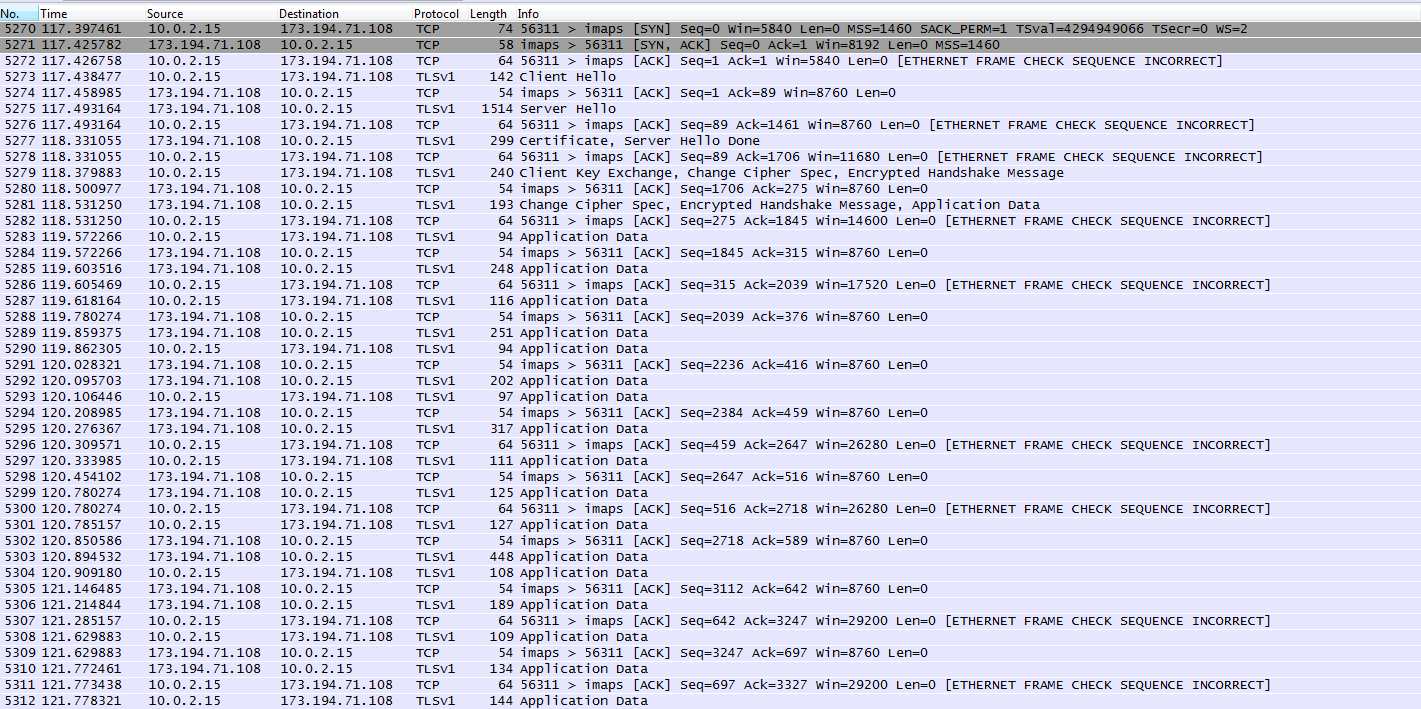
\includegraphics[height=0.6\textwidth, angle=-90]{ws1}
\end{center}
\caption{Traffic going to our application when recieving a single message} \label{fig:ws1}
\end{figure}

\begin{figure}[h!]
\begin{center}
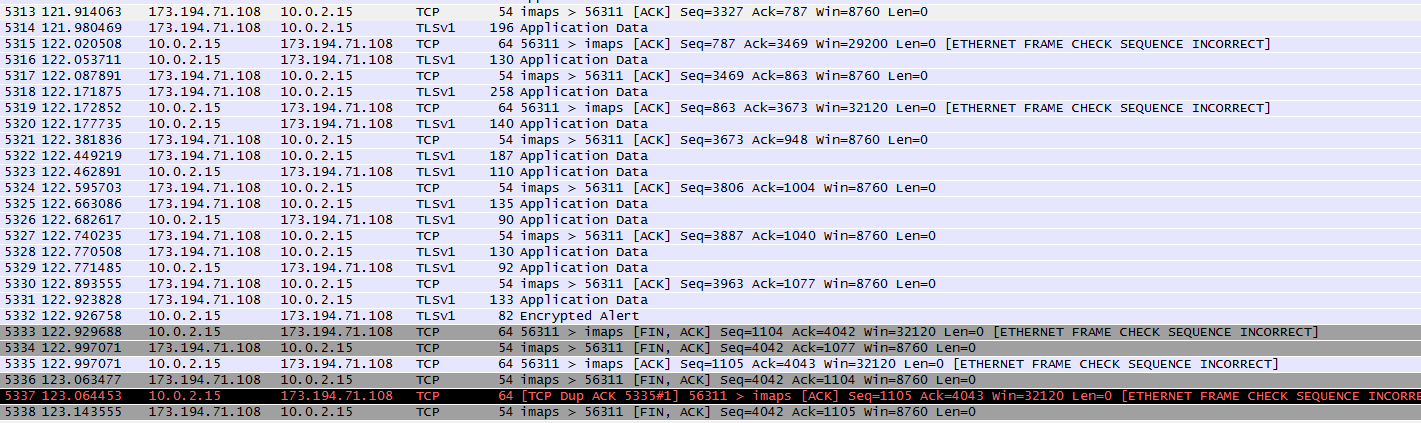
\includegraphics[height=0.38\textwidth, angle=-90]{ws2}
\end{center}
\caption{Traffic going from our application when recieving a single message} \label{fig:ws2}
\end{figure}

\begin{figure}[h!]
\begin{center}
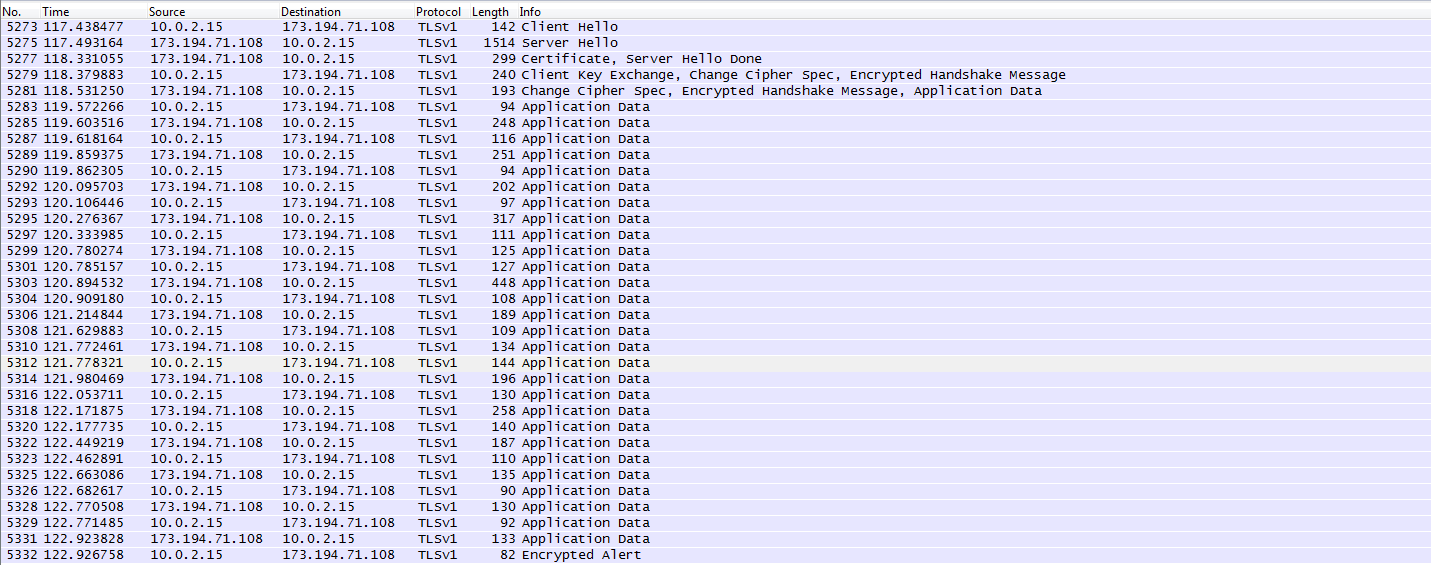
\includegraphics[height=0.5\textwidth, angle=-90]{ws3}
\end{center}
\caption{TLS packets sent to and from our application} \label{fig:ws3}
\end{figure}

\begin{figure}[h!]
\begin{center}
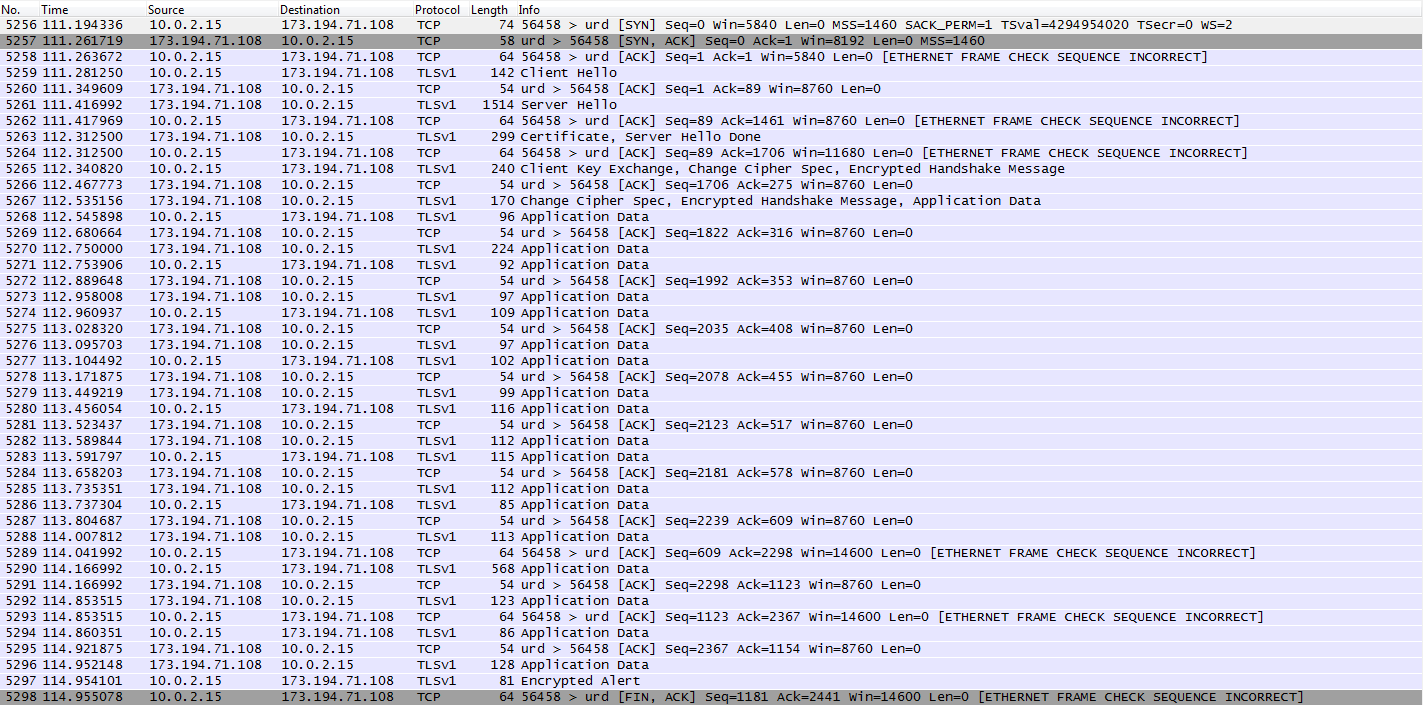
\includegraphics[height=0.6\textwidth, angle=-90]{ws4}
\end{center}
\caption{Traffic going to and from our application when sending a single message from our application} \label{fig:ws4}
\end{figure}

\begin{figure}[h!]
\begin{center}
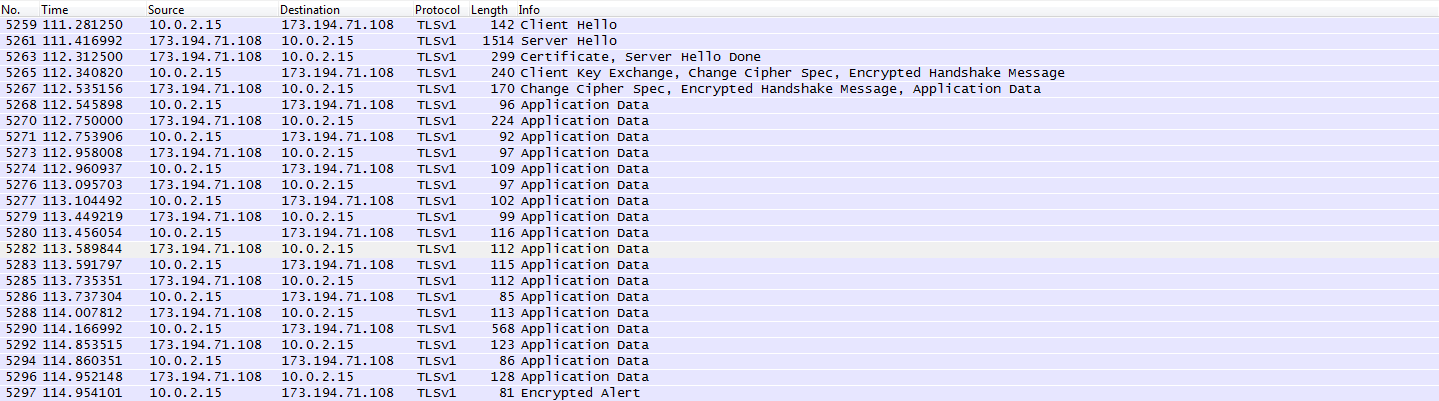
\includegraphics[height=0.35\textwidth, angle=-90]{ws5}
\end{center}
\caption{TLS packets sent to and from our application} \label{fig:ws5}
\end{figure}

	\chapter{Functional tests}\label{ch:funtest}
		See table \ref{tab:case1} - \ref{tab:case28} at page \pageref{tab:case1} - \pageref{tab:case28} for test cases.
		\begin{table}[h!]
			\begin{tabular}{l|p{10cm}}
				Test case ID & 1 \\ \hline
				Name & Login\\ \hline
				Requirement & FR1\\ \hline
				Description & Test the login functionality\\ \hline
				Preconditions & The app has started\\ \hline
				Flow of events & 
					\begin{enumerate}
						\item{}Enter username "kprotesting"
						\item{}Enter password "kprotest"
						\item{}Press login button
					\end{enumerate} \\ \hline
				Expected results & The login screen disappear and the inbox appear\\ \hline
				Actual results & Correct\\ \hline
				Comments & -\\ \hline
				Status & OK\\ \hline
			\end{tabular}
			\caption{Test case 1} \label{tab:case1}
		\end{table}

		\begin{table}[htb]
			\begin{tabular}{l|p{10cm}}
				Test case ID & 2 \\ \hline
				Name & Send regular message\\ \hline
				Requirement & FR2\\ \hline
				Description & Test sending of message with default values\\ \hline
				Preconditions & The user is logged in\\ \hline
				Flow of events & 
					\begin{enumerate}
						\item{}Navigate to the tab for sending a new message
						\item{}Enter email address "kprothales@gmail.com"
						\item{}Enter subject "Hello"
						\item{}Select security label "Unclassified" from the list
						\item{}Enter the text "Hello world!" in the message body area
						\item{}Press send button
					\end{enumerate} \\ \hline
				Expected results & A toast notification that says "Message sent" and sent back to the inbox. The message 						should now be in the "Sent" folder\\ \hline
				Actual results & Correct\\ \hline
				Comments & -\\ \hline
				Status & OK\\ \hline
			\end{tabular}
			\caption{Test case 2} \label{tab:case2}
		\end{table}

		\begin{table}[htb]
			\begin{tabular}{l|p{10cm}}
				Test case ID & 3 \\ \hline
				Name & Send message to contact from the address book\\ \hline
				Requirement & FR2, FR5\\ \hline
				Description & Test sending of message to a contact from the address book\\ \hline
				Preconditions & The user is logged in\\ \hline
				Flow of events & 
					\begin{enumerate}
						\item{}Navigate to the view for sending a new message
						\item{}Press the contacts button
						\item{}Select "kprothales@gmail.com" from the contacts list
						\item{}Enter subject "Hello"
						\item{}Select security label "Unclassified" from the list
						\item{}Press send button
					\end{enumerate} \\ \hline
				Expected results & A toast notification that says "Message sent" and sent back to the inbox. The message 					should now be in the "Sent" folder\\ \hline
				Actual results & Correct\\ \hline
				Comments & -\\ \hline
				Status & OK\\ \hline
			\end{tabular}
			\caption{Test case 3} \label{tab:case3}
		\end{table}

		\begin{table}[htb]
			\begin{tabular}{l|p{10cm}}
				Test case ID & 4 \\ \hline
				Name & Send full message\\ \hline
				Requirement & FR2, FR6\\ \hline
				Description & Test sending of message with attributes set\\ \hline
				Preconditions & The user is logged in\\ \hline
				Flow of events & 
					\begin{enumerate}
						\item{}Navigate to the view for sending a new message
						\item{}Press the contacts button
						\item{}Select "kprothales@gmail.com" from the contacts list
						\item{}Enter subject "Hello"
						\item{}Select security label "Unclassified" from the list
						\item{}Select priority "Deferred"
						\item{}Select type "Exercise"
						\item{}Enter the text "Hello world!" in the message body area
						\item{}Press send button
					\end{enumerate} \\ \hline
				Expected results & A toast notification that says "Message sent" and sent back to inbox. The message 							should now be in the "Sent" folder\\ \hline
				Actual results & Correct\\ \hline
				Comments &-\\ \hline
				Status &OK \\ \hline
			\end{tabular}
			\caption{Test case 4} \label{tab:case4}
		\end{table}

		\begin{table}[htb]
			\begin{tabular}{l|p{10cm}}
				Test case ID & 5 \\ \hline
				Name & Sent messages folder\\ \hline
				Requirement & FR4\\ \hline
				Description & Test sent messages folder\\ \hline
				Preconditions & The user is logged in and at least 3 message has been sent\\ \hline
				Flow of events & 
					\begin{enumerate}
						\item{}Navigate to the view for the folders
						\item{}Change the folder from "Inbox" to "Sent"
						\item{}Press one of the message items
					\end{enumerate} \\ \hline
				Expected results & There should be 3 messages in the folder. The message opens with all the correct 							attributes and text\\ \hline
				Actual results & Correct\\ \hline
				Comments &-\\ \hline
				Status &OK \\ \hline
			\end{tabular}
			\caption{Test case 5} \label{tab:case5}
		\end{table}

		\begin{table}[htb]
			\begin{tabular}{l|p{10cm}}
				Test case ID & 6 \\ \hline
				Name & Read and browse messages\\ \hline
				Requirement & FR3\\ \hline
				Description & Read and browse messages\\ \hline
				Preconditions & The user is logged in and there are at least two message in the inbox folder\\ \hline
				Flow of events & 
					\begin{enumerate}
						\item{}Navigate to the folders view and look in the inbox folder
						\item{}Press a message in the message list
						\item{}Browse between the messages (to previous and/or next message)
					\end{enumerate} \\ \hline
				Expected results & The message view appears and shows the sender, subject, security label, priority, 							type, attachments if any and the message body. The message view changes the fields according to 						what message the user is viewing \\ \hline
				Actual results & Correct\\ \hline
				Comments & -\\ \hline
				Status & OK\\ \hline
			\end{tabular}
			\caption{Test case 6} \label{tab:case6}
		\end{table}

		\begin{table}[htb]
			\begin{tabular}{l|p{10cm}}
				Test case ID & 7 \\ \hline
				Name & Send attachment (camera)\\ \hline
				Requirement & FR7\\ \hline
				Description & Test sending of image from camera\\ \hline
				Preconditions & The user is logged in\\ \hline
				Flow of events & 
					\begin{enumerate}
						\item{}Navigate to the view for sending a new message
						\item{}Press the contacts button
						\item{}Select "kprotesting@gmail.com" (yourself) from the contacts list
						\item{}Enter subject "Hello"
						\item{}Select security label "Unclassified" from the list
						\item{}Press the button for adding an attachment
						\item{}Take a picture with the camera
						\item{}Press the send button
					\end{enumerate} \\ \hline
				Expected results & A toast notification that says "Message sent" and sent back to inbox\\ \hline
				Actual results & Correct\\ \hline
				Comments & -\\ \hline
				Status &OK \\ \hline
			\end{tabular}
			\caption{Test case 7} \label{tab:case7}
		\end{table}

		\begin{table}[htb]
			\begin{tabular}{l|p{10cm}}
				Test case ID & 8 \\ \hline
				Name & Send attachment (gallery)\\ \hline
				Requirement & FR7\\ \hline
				Description & Test sending of image from gallery\\ \hline
				Preconditions & The user is logged in and has at least one image in the gallery\\ \hline
				Flow of events & 
					\begin{enumerate}
						\item{}Navigate to the view for sending a new message
						\item{}Press the contacts button
						\item{}Select "kprotesting@gmail.com" (yourself) from the contacts list
						\item{}Enter subject "Hello"
						\item{}Select security label "Unclassified" from the list
						\item{}Press the button for adding an attachment
						\item{}Select an image from the gallery
						\item{}Press the send button
					\end{enumerate} \\ \hline
				Expected results & A toast notification that says "Message sent" and sent back to inbox\\ \hline
				Actual results & Correct\\ \hline
				Comments & -\\ \hline
				Status &OK \\ \hline
			\end{tabular}
			\caption{Test case 8} \label{tab:case8}
		\end{table}

		\begin{table}[htb]
			\begin{tabular}{l|p{10cm}}
				Test case ID & 9 \\ \hline
				Name & Send attachment (GPS)\\ \hline
				Requirement & FR7\\ \hline
				Description & Test sending of GPS coordinates\\ \hline
				Preconditions & The user is logged in\\ \hline
				Flow of events & 
					\begin{enumerate}
						\item{}Navigate to the view for sending a new message
						\item{}Press the contacts button
						\item{}Select "kprotest@gmail.com" (yourself) from the contacts list
						\item{}Enter subject "Hello"
						\item{}Select security label "Unclassified" from the list
						\item{}Press the button for adding an attachment
						\item{}Add location (GPS-coordinates)
						\item{}Press the send button
					\end{enumerate} \\ \hline
				Expected results & The message text should be filled out with the current location. A toast notification that says "Message sent" and sent back to inbox\\ \hline
				Actual results &Correct\\ \hline
				Comments &-\\ \hline
				Status &OK\\ \hline
			\end{tabular}
			\caption{Test case 9} \label{tab:case9}
		\end{table}

		\begin{table}[htb]
			\begin{tabular}{l|p{10cm}}
				Test case ID & 10 \\ \hline
				Name & Attachments received\\ \hline
				Requirement & FR7\\ \hline
				Description & Test reading and opening of a message with attachments\\ \hline
				Preconditions & The user is logged in and there is at least one message with attachements\\ \hline
				Flow of events & 
					\begin{enumerate}
						\item{}Navigate to the folders and make sure you view inbox messages
						\item{}Press a message that has an attachment (e.g. one of the messages you sent to yourself in previous tests)
						\item{}Press the button to show the attachments
						\item{}Open the image that is attached
					\end{enumerate} \\ \hline
				Expected results & The correct program for opening an image is started and the image is shown \\ \hline
				Actual results &Correct\\ \hline
				Comments &-\\ \hline
				Status &OK \\ \hline
			\end{tabular}
			\caption{Test case 10} \label{tab:case10}
		\end{table}

		\begin{table}[htb]
			\begin{tabular}{l|p{10cm}}
				Test case ID & 11 \\ \hline
				Name & Instant message settings\\ \hline
				Requirement & FR9, FR10\\ \hline
				Description & Test instant message settings\\ \hline
				Preconditions & The user is logged in\\ \hline
				Flow of events & 
					\begin{enumerate}
						\item{}Navigate to the settings view and view the settings for instant message attributes
						\item{}Set "kprothales@gmail.com" as standard receiver
						\item{}Set "Restricted" as standard security label
						\item{}Set "Flash" as standard priority
						\item{}Set "Drill" as standard type
						\item{}Navigate back to the instant message view
					\end{enumerate} \\ \hline
				Expected results & The instant message view should have fields corresponding to the settings chosen \\ \hline
				Actual results &Correct\\ \hline
				Comments &-\\ \hline
				Status & OK\\ \hline
			\end{tabular}
			\caption{Test case 11} \label{tab:case11}
		\end{table}

		\begin{table}[htb]
			\begin{tabular}{l|p{10cm}}
				Test case ID & 12\\ \hline
				Name & Message retrival strategy settings\\ \hline
				Requirement & FR10\\ \hline
				Description & Test settings for push/pull strategy\\ \hline
				Preconditions & The user is logged in\\ \hline
				Flow of events & 
					\begin{enumerate}
						\item{}Navigate to the settings view and view the settings for message retrieval
						\item{}Change the strategy to "pull"
						\item{}Set the poll interval to 1 minute
					\end{enumerate} \\ \hline
				Expected results & The app should now change strategy from push (default) to pull \\ \hline
				Actual results & The app still uses push strategy\\ \hline
				Comments & Unknown, has tried to debug\\ \hline
				Status & Failed\\ \hline
			\end{tabular}
			\caption{Test case 12} \label{tab:case12}
		\end{table}

		\begin{table}[htb]
			\begin{tabular}{l|p{10cm}}
				Test case ID & 13\\ \hline
				Name & Security labels settings\\ \hline
				Requirement & FR10\\ \hline
				Description & Test settings for available security labels\\ \hline
				Preconditions & The user is logged in\\ \hline
				Flow of events & 
					\begin{enumerate}
						\item{}Navigate to the settings view and view the settings for security labels
						\item{}Check the checkboxes for "RESTRICTED" and "NATO UNCLASSIFIED"
						\item{}Uncheck the rest
						\item{}Navigate to the send message view
					\end{enumerate} \\ \hline
				Expected results & The dropdown list of security labels should be filled out according to the choices in the settings \\ \hline
				Actual results &All the security labels are still shown\\ \hline
				Comments & Known deficiency, has not been implemented\\ \hline
				Status &Failed\\ \hline
			\end{tabular}
			\caption{Test case 13} \label{tab:case13}
		\end{table}

		\begin{table}[htb]
			\begin{tabular}{l|p{10cm}}
				Test case ID & 14 \\ \hline
				Name & Send instant message\\ \hline
				Requirement & FR9\\ \hline
				Description & Test sending of an instant message\\ \hline
				Preconditions & The user is logged in\\ \hline
				Flow of events & 
					\begin{enumerate}
						\item{}Navigate to the instant message view
						\item{}Enter the text "Hello World" in the message body text area
						\item{}Press the send button
					\end{enumerate} \\ \hline
				Expected results & The fields in the view are filled out according to the settings. The message is sent instantly. Toast notification that says "Message sent" and sent back to the inbox \\ \hline
				Actual results & Correct\\ \hline
				Comments &-\\ \hline
				Status &OK \\ \hline
			\end{tabular}
			\caption{Test case 14} \label{tab:case14}
		\end{table}

		\begin{table}[htb]
			\begin{tabular}{l|p{10cm}}
				Test case ID & 15 \\ \hline
				Name & Receive of an flash/override message\\ \hline
				Requirement & TODO\\ \hline
				Description & Test receiving of an high priority message\\ \hline
				Preconditions & The user is logged in and someone has sent a high-priority message to the user\\ \hline
				Flow of events & 
					\begin{enumerate}
						\item{}A red box takes over the screen
						\item{}Click open message
					\end{enumerate} \\ \hline
				Expected results & The message is shown in the regular message view\\ \hline
				Actual results & Correct\\ \hline
				Comments & -\\ \hline
				Status & OK \\ \hline
			\end{tabular}
			\caption{Test case 15} \label{tab:case15}
		\end{table}

		\begin{table}
			\begin{tabular}{l|p{10cm}}
				Test case ID & 16 \\ \hline
				Name & Send instant message with attachments\\ \hline
				Requirement & FR9\\ \hline
				Description & Test sending of instant message with attachments\\ \hline
				Preconditions & The user is logged in and has at least one image in the gallery\\ \hline
				Flow of events & 
					\begin{enumerate}
						\item{}Navigate to the instant message view
						\item{}Check if the predefined values are set (if not set them in settings)
						\item{}Press the button for add attachment
						\item{}Select an image from the gallery
						\item{}Press the button for adding attachment again	
						\item{}Add GPS coordinates to the message
						\item{}Press the send button
					\end{enumerate} \\ \hline
				Expected results & The message is sent instantly.  Toast notification that says "Message sent" and sent 							back to the inbox\\ \hline
				Actual results &GPS coordinates is attached, but the message attributes somehow get wrong\\ \hline
				Comments &Unknown\\ \hline
				Status &Image OK, GPS failed\\ \hline
			\end{tabular}
			\caption{Test case 16} \label{tab:case16}
		\end{table}

		\begin{table}
			\begin{tabular}{l|p{10cm}}
				Test case ID & 17 \\ \hline
				Name & Receive instant message outside the application\\ \hline
				Requirement & TODO\\ \hline
				Description & Test receiving of instant message outside the application\\ \hline
				Preconditions & The user is logged in and the application is in the background\\ \hline
				Flow of events & 
					\begin{enumerate}
						\item{}A red box takes over the screen
						\item{}Click open message
					\end{enumerate} \\ \hline
				Expected results & The message is shown in the regular message view\\ \hline
				Actual results &Correct\\ \hline
				Comments &-\\ \hline
				Status & OK\\ \hline
			\end{tabular}
			\caption{Test case 17} \label{tab:case17}
		\end{table}

		\begin{table}
			\begin{tabular}{l|p{10cm}}
				Test case ID & 18 \\ \hline
				Name & Widget for instant message\\ \hline
				Requirement & FR9\\ \hline
				Description & Test the widget for sending an instant message\\ \hline
				Preconditions & The user is logged in and the widget is placed on the home screen\\ \hline
				Flow of events & 
					\begin{enumerate}
						\item{}Click the widget
					\end{enumerate} \\ \hline
				Expected results & The app opens and the view for sending an instant message is opened\\ \hline
				Actual results & Correct\\ \hline
				Comments &-\\ \hline
				Status &OK \\ \hline
			\end{tabular}
			\caption{Test case 18} \label{tab:case18}
		\end{table}

		\clearpage

		\begin{table}
			\begin{tabular}{l|p{10cm}}
				Test case ID & 19 \\ \hline
				Name & Reply\\ \hline
				Requirement & FR8\\ \hline
				Description & Test reply of a message\\ \hline
				Preconditions & The user is logged in and has at least one message in the inbox\\ \hline
				Flow of events & 
					\begin{enumerate}
						\item{}Navigate to the folders view and look at the inbox
						\item{}Click on a message in the list
						\item{}Press the reply button
					\end{enumerate} \\ \hline
				Expected results & The send message view opens with the correct fields filled out, the security label is fixed and "Re:" stands before the subject. \\ \hline
				Actual results &The correct actions happen, but one gets sent out of the tab system\\ \hline
				Comments & This feature has not been implemented perfect\\ \hline
				Status & OK-\\ \hline
			\end{tabular}
			\caption{Test case 19} \label{tab:case19}
		\end{table}

		\begin{table}
			\begin{tabular}{l|p{10cm}}
				Test case ID & 20 \\ \hline
				Name & Forward\\ \hline
				Requirement &FR8\\ \hline
				Description & Test forwarding of a message\\ \hline
				Preconditions & The user is logged in and has at least one message in the inbox\\ \hline
				Flow of events & 
					\begin{enumerate}
						\item{}Navigate to the folders view and look at the inbox
						\item{}Click on a message in the list
						\item{}Press the forward button
					\end{enumerate} \\ \hline
				Expected results & The send message view opens with the correct fields filled out, the security label is fixed and "Fwd:" before the subject. \\ \hline
				Actual results & The correct actions happen, but one gets sent out of the tab system\\ \hline
				Comments & OK-\\ \hline
				Status & \\ \hline
			\end{tabular}
			\caption{Test case 20} \label{tab:case20}
		\end{table}

		\begin{table}
			\begin{tabular}{l|p{10cm}}
				Test case ID & 21 \\ \hline
				Name & Delete\\ \hline
				Requirement & FR8\\ \hline
				Description & Test deleting of a message\\ \hline
				Preconditions & The user is logged in and has at least one message in the inbox\\ \hline
				Flow of events & 
					\begin{enumerate}
						\item{}Navigate to the folders view and look at the inbox
						\item{}Click on a message in the list
						\item{}Press the menu button
						\item{}Press delete on the popup menu that shows at the lower part of the screen
					\end{enumerate} \\ \hline
				Expected results & The view changes to the inbox and the message has disappeared from the list. \\ \hline
				Actual results &The message disappears at first, but is still there if you log out and in\\ \hline
				Comments &Known deficiency, problems with the Android file system\\ \hline
				Status &Failed \\ \hline
			\end{tabular}
			\caption{Test case 21} \label{tab:case21}
		\end{table}

		\begin{table}
			\begin{tabular}{l|p{10cm}}
				Test case ID & 22 \\ \hline
				Name & Delivery report and receipt notification\\ \hline
				Requirement & TODO\\ \hline
				Description & Test sending of a message where one has requested delivery report and receipt notification\\ \hline
				Preconditions & The user is logged in\\ \hline
				Flow of events & 
					\begin{enumerate}
						\item{}Navigate to the send message view
						\item{}Set "kprothales@gmail.com" as receiver
						\item{}Set "Hello world" as subject
						\item{}Set "UNCLASSIFIED" as security label
						\item{}Enter "Hello everybody" in the message text.
						\item{}Request delivery report and receipt notification
						\item{}Press the send button
					\end{enumerate} \\ \hline
				Expected results & A toast notification that says "Message sent" and sent back to inbox \\ \hline
				Actual results & Feature not implemented\\ \hline
				Comments &Feature not implemented\\ \hline
				Status &Failed \\ \hline
			\end{tabular}
			\caption{Test case 22} \label{tab:case22}
		\end{table}

		\begin{table}
			\begin{tabular}{l|p{10cm}}
				Test case ID & 23 \\ \hline
				Name & Status of delivery report and receipt notification\\ \hline
				Requirement &TODO\\ \hline
				Description & Test checking status on a message where one has requested delivery report and receipt notification\\ \hline
				Preconditions & The user is logged in and has at least one sent message that has a request for delivery report and receipt notification\\ \hline
				Flow of events & 
					\begin{enumerate}
						\item{}Navigate to the sent messages
						\item{}Click on a message that has a request for delivery report and receipt notification
						\item{}View the status of the delivery report and receipt notification
					\end{enumerate} \\ \hline
				Expected results & The message has fields with these attributes, which is red at first but changes to green when the status is updated to deliverd/read \\ \hline
				Actual results &Not implemented\\ \hline
				Comments & Not implemented\\ \hline
				Status & Failed\\ \hline
			\end{tabular}
			\caption{Test case 23} \label{tab:case23}
		\end{table}

		\begin{table}
			\begin{tabular}{l|p{10cm}}
				Test case ID & 24 \\ \hline
				Name & Sort\\ \hline
				Requirement & 3TODO\\ \hline
				Description & Test sorting of messages in the inbox based on different criterias\\ \hline
				Preconditions & The user is logged in and has at least 4 different messages in the inbox\\ \hline
				Flow of events & 
					\begin{enumerate}
						\item{}Navigate to folders view 
						\item{}Press the sort button and choose different sorting algorithms
					\end{enumerate} \\ \hline
				Expected results & The inbox messages are sorted correct according to the sorting criteria\\ \hline
				Actual results &Correct\\ \hline
				Comments &-\\ \hline
				Status &OK \\ \hline
			\end{tabular}
			\caption{Test case 24} \label{tab:case24}
		\end{table}

		\begin{table}
			\begin{tabular}{l|p{10cm}}
				Test case ID & 25 \\ \hline
				Name & Search\\ \hline
				Requirement & TODO\\ \hline
				Description & Test searching of messages in folders\\ \hline
				Preconditions & The user is logged in and has at least 4 different messages in the inbox\\ \hline
				Flow of events & 
					\begin{enumerate}
						\item{}Navigate to folders view 
						\item{}Enter text in the search field and press Enter
					\end{enumerate} \\ \hline
				Expected results & The folder is filtrated to show only the items that match the search condition\\ \hline
				Actual results & Not implemented\\ \hline
				Comments & Not implemented\\ \hline
				Status & Failed\\ \hline
			\end{tabular}
			\caption{Test case 25} \label{tab:case25}
		\end{table}

			\begin{table}
			\begin{tabular}{l|p{10cm}}
				Test case ID & 26\\ \hline
				Name & Login incorrect input\\ \hline
				Requirement & FR1\\ \hline
				Description&Test how the app reacts to incorrect login input\\ \hline
				Preconditions&The app has started\\ \hline
				Tasks&\begin{enumerate}
						\item{}Enter bogus username and password
						\item{}Leave the username field empty
						\item{}Leave the password field empty
						\item{}Leave both fields empty
					\end{enumerate} \\ \hline
				Expected result&An error message showing "Incorrect login information" and the user do not get logged in\\ \hline
				Actual result& Tasks 1-4 gives the correct error message and the login is not allowed\\ \hline
				Comments&- \\ \hline
				Status& OK\\ \hline 
			\end{tabular}
			\caption{Test case 26} \label{tab:case26}
			\end{table}

				\begin{table}
			\begin{tabular}{l|p{10cm}}
				Test case ID & 27\\ \hline
				Name & Receiver incorrect input\\ \hline
				Requirement & FR2\\ \hline
				Description&Test how the app reacts to incorrect receiver input\\ \hline
				Preconditions&The user is logged in and looks at the send message view\\ \hline
				Tasks&\begin{enumerate}
						\item{}Leave the receiver field empty
						\item{}Enter several words with an arbitrary separator
					\end{enumerate} \\ \hline
				Expected result&A validation error message in the text field that says "The address is not valid. Please check again". \\ \hline
				Actual result&Tasks 1-2 correct\\ \hline
				Comments&-\\ \hline
				Status& OK\\ \hline 
			\end{tabular}
			\caption{Test case 27} \label{tab:case27}
			\end{table}

				\begin{table}
			\begin{tabular}{l|p{10cm}}
				Test case ID & 28\\ \hline
				Name &Security label incorrect input\\ \hline
				Requirement & FR2\\ \hline
				Description&Test how the app reacts to incorrect security label input\\ \hline
				Preconditions&The user is logged in and looks at the send message view\\ \hline
				Tasks&\begin{enumerate}
						\item{}Do net set a value for the security label
					\end{enumerate} \\ \hline
				Expected result&An error message showing "You need to set a security label" and the message does not get sent\\ \hline
				Actual result& Correct\\ \hline
				Comments&- \\ \hline
				Status& OK\\ \hline 
			\end{tabular}
			\caption{Test case 28} \label{tab:case28}
			\end{table}

	\documentclass[a4paper,12pt]{article}
\usepackage{array}
\usepackage{pdfpages}
\begin{document}
\section{Usability testing}
	\subsection{Test execution}
		\subsubsection{Preparation for the test leader}
			\begin{itemize}
				\item{}Make sure you have the latest version of XOXOmail (updated 08.11) installed and Internet connection on your phone/computer
				\item{}Have the tasks ready on paper or screen
				\item{}Have the SUS questionnaire ready on paper or screen
				\item{}Have pen and the observation form on paper or a computer ready to make notes on
				\item{}Preconditions for the tests: Make sure there are no mails on the account (kprotesting@gmail.com/kprotest) with flash/override as priority. Other messages are OK.
				\item{}Put an ID (e.g. the test leader's name) on both the observation form and the SUS questionnaire. 
				\item{}Note that task 5 is meant to open the message the test person sent to himself/herself. If the test person sent the message to another address or failed to send a message, you need to send a new message with flash/override priority to kprotesting@gmail.com.
			\end{itemize}
		
		\subsubsection{Information about the test given to the user}
			\begin{itemize}
				\item{}This is a test to find out if the app is intuitive and user friendly, and not a test of you and your skills.
				\item{}The test consists of six (6) tasks and will take approximately 20 minutes.
				\item{}Read the instructions for each task and perform the tasks one by one.
				\item{}Each task has the same structure: A task number, a task name, a description of what you should do and input data that is needed to solve a task. If you find input fields in the app that do not have a value listed, you can enter an arbitrary value.
				\item{}If you cannot figure out how to solve a task this is not your fault, but the app that is not designed in a user friendly way. You can then move on to the next task, but notify the test leader.
				\item{}You can ask questions before and after the test, but we cannot help you during the test.
				\item{}You can quit the test anytime you want.
				\item{}It would be helpful if you could try to think aloud during the test. Try to explain what you see and why you make your choices. This makes it easier for us to figure out how users think and what could be done better in the design.
				\item{}After the test we would appreciate if you could fill out a questionnaire and give feedback if you felt that something worked well or not so well.
			\end{itemize}
\subsubsection{Information about the app given to the user}
			XOXOmail is a mail client app for Android phones. It is intended for use in the military or other similar organizations. The app is very much like a regular mail client app, but the difference is that a mail in this app can be given three special  attributes: security label, priority and type. Otherwise the app has the ability, like regular mail clients, to send and receive messages with and without attachments. 
			\newline
			\newline
			There is also a distinction between a regular mail and a so-called instant message. An instant message is meant for quicker sending, where you can predefine a receiver and values of the three attributes in the settings.  A last thing to note is that messages with high priority are handled differently from regular messages, as they will take over the screen and force an action to either open the message or cancel to carry on with what you were doing.
	     	\subsubsection{SUS form}
			The SUS form can be found in figure \ref{fig:SUS_form} on page \pageref{fig:SUS_form}
			\begin{figure}[htp]{
			\includegraphics[page=4, scale=0.8]{./SUS_info.pdf}}
			\caption{SUS form}\label{fig:SUS_form}
			\end{figure}
		\subsubsection{Observation form}
			The observation form template can be found in figure \ref{fig:observation_form} on page \pageref{fig:observation_form}
			\begin{figure}[htp]{
			\includegraphics[scale=0.8]{./observation_form.pdf}}
			\caption{Observation form}\label{fig:observation_form}
			\end{figure}
	\subsection{The results}
	\includepdf[pages={1,2,3,4,5}]{./observation_form_results.pdf}
\end{document}

	\chapter{User manual}


	\chapter{User manual}


   \begin{center}
    \vspace*{3\baselineskip}
    \large
    \bfseries
    XOXOmail\\[2\baselineskip]
    
    User Manual \\
    \normalfont
    \large
    
    	
    
\includegraphics[height=18em]{login_screen}
  \end{center}

\newpage

\section*{Contents}
\begin{enumerate}
\item{}Logging in
\item{}Viewing the inbox
\item{}Sending a message
\item{}Instant messages
\item{}Flash and Override messages
\item{}Configuring the settings
\end{enumerate}

\newpage
\section*{Logging in}

After starting the XOXOmail application you will be prompted with a login screen. In order to login, simply press the login button below the password field. There is no need to enter any information in the Email and Password field as this has not yet been implemented. 

  \begin{center}
    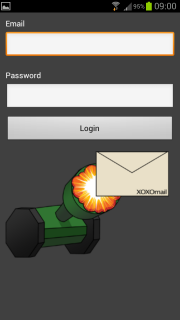
\includegraphics{logingui1}
  \end{center}
  \newpage
  
\section*{Viewing the inbox}
To view the inbox, make sure the inbox tab i selected. You will then see a list of all messages currently in the inbox. If you want to sort these messages, simply press the sort button indicated in the screenshot below.   

  \begin{center}
    \includegraphics{viewinboxarrows}
  \end{center}
\newpage
You can then select the desired sorting algorithm by pressing the different options presented. 
  \begin{center}
    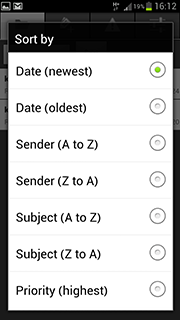
\includegraphics{SortBy}
  \end{center}

\newpage
If you want to view any of the messages currently in the inbox, you can press the messages displayed on the screen. You will then be brought to the message view. 
\newline 
\newline 
From the message view you can see the sender of the message, the message attributes and the actual message text. You also have the opportunity to change between received messages, reply to a message and forward the received message. This is done by pressing the respective buttons at the bottom of the screen.

  \begin{center}
    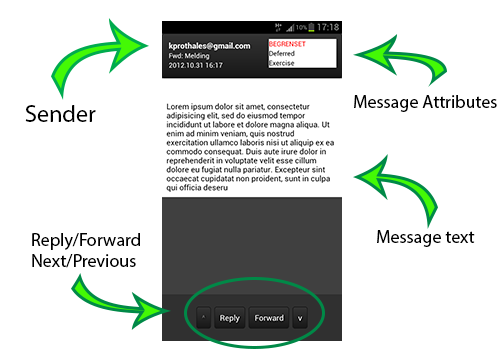
\includegraphics{ViewMessageArrows}
  \end{center}

\newpage
\section*{Sending a message}
To send a new message, you must first make sure you have the send message tab selected. You will then be presented with the send message view. \newline \newline First you must select the recipient of the message to be sent. This can be done by either typing in the recipient manually or pressing the contacts button.  
  \begin{center}
    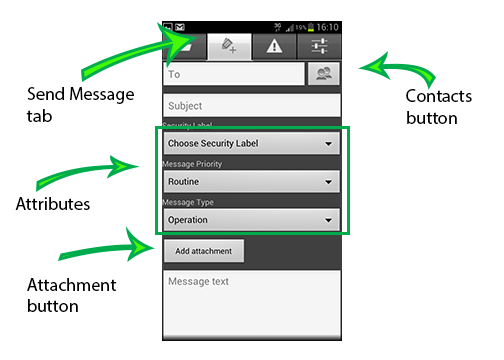
\includegraphics{sendmessagearrows}
  \end{center}
  \newpage
  If the contacts button is pressed, a new window will open displaying your contacts. Pressing one of these contacts will add the address to the "To" field.
  \begin{center}
    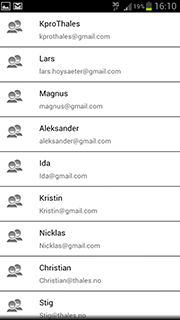
\includegraphics{Contacts1}
  \end{center}
\newpage
After choosing a recipient you must add a subject to your message. This is done by typing in the subject in the field below the recipient field.
\newline 
\newline 
The next step is to select which attributes your message will include. You will need to select the label, priority and type of the message, if the attributes are not selected, the default values will be added to the message. 

\begin{figure}[h]
\makebox[\textwidth]{%
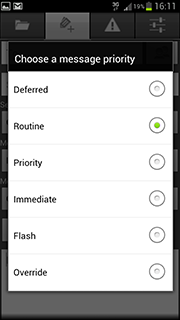
\includegraphics[width=0.30\textwidth]{ChooseMessagePriority}%
\hfill    
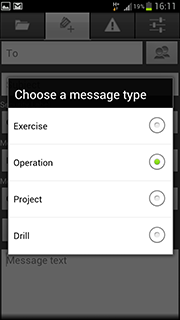
\includegraphics[width=0.30\textwidth]{ChooseMessageType}%
\hfill    
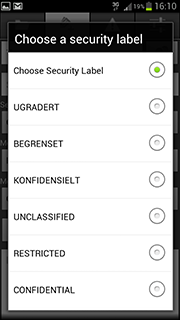
\includegraphics[width=0.30\textwidth]{ChooseSecurityLabelz}%
}%
\caption{Choosing attributes}
\label{fig:OlimpicCircleTT1}
\end{figure}

\newpage
After adding the message attributes you have the opportunity to add an attachment to your message. This can be an image from the camera, an image already stored on the phone or your current GPS location. 

 \begin{center}
    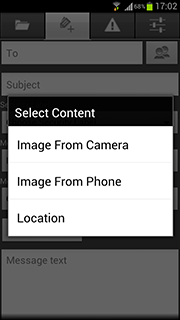
\includegraphics{attachments}
  \end{center}

Finally the actual message text can be added to the message. This is done by pressing the Message text field and typing in the desired text. To send your message, simply press the send button at the bottom of the screen. 
\newpage
\subsubsection{Instant messages}
To send an instant message, you must have the instant message tab selected. The instant message view shows you the predefined recipient and attributes. The predefined values are set in the settings menu. To send an instant message you simply type in the message text and press the send button. 
 \begin{center}
    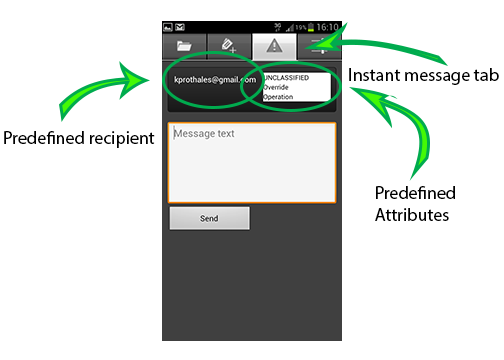
\includegraphics{instantmessagearrows}
  \end{center}


\newpage
\section*{Flash and Override messages}




When receiving a message with message priority set to Flash or Override, a red popup will cover your screen. You can then view this message, or press cancel to close the window.

 \begin{center}
    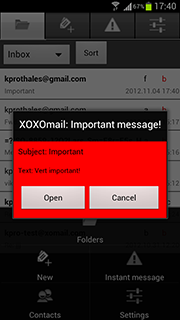
\includegraphics{FLASH}
  \end{center}


\newpage
\section*{Configuring the settings}

To alter the various settings in the application, you must have the settings tab selected.
 \begin{center}
    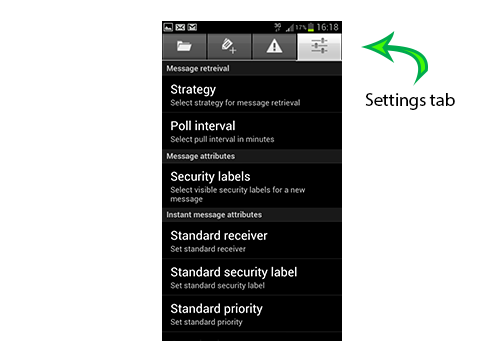
\includegraphics{settingsarrow}
  \end{center}

In the settings tab you have 4 different categories of configurable settings:
\begin{itemize}
\item{}Message retrieval
\item{}Message attributes
\item{}Instant message attributes
\item{}Location data
\end{itemize}

\newpage
In the message retrieval section you have the ability to choose the message retrieval strategy and poll interval. 
\newline 
\newline
There are 2 message retrieval strategies available at this time: push and pull. When pull is selected, the messages in the inbox are loaded every given interval. The application queries the server for new messages after a set interval has passed. \newline 
If push is selected the application will load all the messages in the inbox after startup. When a new message arrives the server will push the message to the application and display it in the inbox. 

\begin{figure}[h]
\makebox[\textwidth]{%
\hfill  
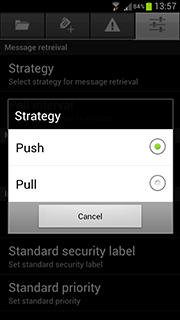
\includegraphics[width=0.40\textwidth]{PullStrategy}%
\hfill    
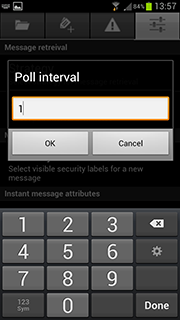
\includegraphics[width=0.40\textwidth]{PollInterval}%
\hfill    

}%
\caption{Pull strategy and poll interval}
\label{fig:OlimpicCircleTT1}
\end{figure}
 
\newpage
In the message attributes section you have the ability to select which attributes that you would like to choose amongst when sending a message.
   \begin{center}
    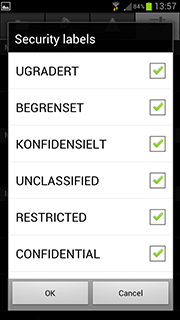
\includegraphics{SecurityLabelsShown}
  \end{center}
\newpage
In the instant message attributes section you have the ability to set the different standard values for sending an instant message. These include:

\begin{itemize}
\item{}Standard receiver
\item{}Standard security label
\item{}Standard priority
\item{}Standard type
\end{itemize}

\begin{figure}[h]
\makebox[\textwidth]{%
\hfill  
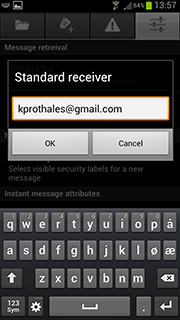
\includegraphics[width=0.24\textwidth]{StandardReceiver}%
\hfill    
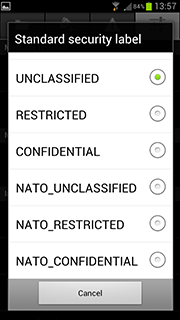
\includegraphics[width=0.24\textwidth]{StandardSecurityLabel}%
\hfill    
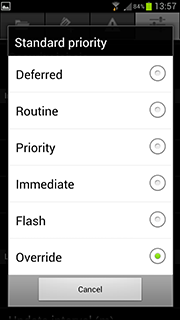
\includegraphics[width=0.24\textwidth]{StandardPriority}%
\hfill    
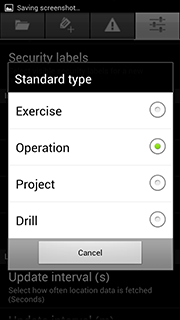
\includegraphics[width=0.24\textwidth]{StandardType}%
\hfill   
}%
\caption{Instant message standard values}
\label{fig:OlimpicCircleTT1}
\end{figure}

\newpage
In the location data section you can choose when the gps position is fetched. This is done by setting how often it should try to update the gps position in seconds, and also how far you need to travel in order update the gps coordinates. 

\begin{figure}[h]
\makebox[\textwidth]{%
\hfill  
\includegraphics[width=0.49\textwidth]{GPSUpdateInterval}%
\hfill    
\includegraphics[width=0.49\textwidth]{GPSUpdateIntervalMeters}%
\hfill    

}%
\caption{GPS settings}
\label{fig:OlimpicCircleTT1}
\end{figure}



	\chapter{Templates}

\section{Agendas}

\begin{figure}[htb]

\includepdf[pages=1]{YYYY-MM-DD-Agenda-Advisor.pdf}

\end{figure}

\newpage

\begin{figure}[htb]

\includepdf[pages=2]{YYYY-MM-DD-Agenda-Advisor.pdf}

\end{figure}

\newpage

\begin{figure}[htb]

\includepdf[pages=-]{YYYY-MM-DD-Agenda-Customer.pdf}

\end{figure}

\newpage

\begin{figure}[htb]

\includepdf[pages=-]{YYYY-MM-DD-Agenda-Internal.pdf}

\end{figure}

\newpage

\section{Weekly Status Report}

\begin{figure}[htb]

\includepdf[pages=-]{YYYY-MM-DD-WeeklyStatusReport-WeekWW.pdf}

\end{figure}

\newpage

\section{Minutes}

\begin{figure}[htb]

\includepdf[pages=1]{YYYY-MM-DD-Minutes-Advisor.pdf}

\end{figure}

\newpage

\begin{figure}[htb]

\includepdf[pages=2]{YYYY-MM-DD-Minutes-Advisor.pdf}

\end{figure}

\newpage

\begin{figure}[htb]

\includepdf[pages=1]{YYYY-MM-DD-Minutes-Customer.pdf}

\end{figure}

\newpage

\begin{figure}[htb]

\includepdf[pages=2]{YYYY-MM-DD-Minutes-Customer.pdf}

\end{figure}

\newpage

\begin{figure}[htb]

\includepdf[pages=-]{YYYY-MM-DD-Minutes-Internal.pdf}

\end{figure}



	\chapter{Agendas}

\section{Advisor}
The following pages include all agendas for advisor meetings.
\newpage
\begin{figure}[htb]
\includepdf[pages=1]{2012-09-04-Agenda-Advisor.pdf}
\end{figure}

\newpage

\begin{figure}[htb]
\includepdf[pages=2]{2012-09-04-Agenda-Advisor.pdf}
\end{figure}

\newpage

\begin{figure}[htb]
\includepdf[pages=3]{2012-09-04-Agenda-Advisor.pdf}
\end{figure}

\newpage

\begin{figure}[htb]
\includepdf[pages=1]{2012-09-20-Agenda-Advisor.pdf}
\end{figure}

\newpage

\begin{figure}[htb]
\includepdf[pages=2]{2012-09-20-Agenda-Advisor.pdf}
\end{figure}

\newpage

\begin{figure}[htb]
\includepdf[pages=1]{2012-09-25-Agenda-Advisor.pdf}
\end{figure}

\newpage

\begin{figure}[htb]
\includepdf[pages=2]{2012-09-25-Agenda-Advisor.pdf}
\end{figure}

\newpage

\begin{figure}[htb]
\includepdf[pages=1]{2012-10-02-Agenda-Advisor.pdf}
\end{figure}

\newpage

\begin{figure}[htb]
\includepdf[pages=2]{2012-10-02-Agenda-Advisor.pdf}
\end{figure}

\newpage

\begin{figure}[htb]
\includepdf[pages=1]{2012-10-09-Agenda-Advisor.pdf}
\end{figure}

\newpage

\begin{figure}[htb]
\includepdf[pages=2]{2012-10-09-Agenda-Advisor.pdf}
\end{figure}

\newpage

\begin{figure}[htb]
\includepdf[pages=1]{2012-10-16-Agenda-Advisor.pdf}
\end{figure}

\newpage

\begin{figure}[htb]
\includepdf[pages=2]{2012-10-16-Agenda-Advisor.pdf}
\end{figure}

\newpage

\begin{figure}[htb]
\includepdf[pages=1]{2012-10-23-Agenda-Advisor.pdf}
\end{figure}

\newpage

\begin{figure}[htb]
\includepdf[pages=2]{2012-10-23-Agenda-Advisor.pdf}
\end{figure}

\newpage

\begin{figure}[htb]
\includepdf[pages=1]{2012-10-30-Agenda-Advisor.pdf}
\end{figure}

\newpage

\begin{figure}[htb]
\includepdf[pages=2]{2012-10-30-Agenda-Advisor.pdf}
\end{figure}

\newpage

\begin{figure}[htb]
\includepdf[pages=1]{2012-11-06-Agenda-Advisor.pdf}
\end{figure}

\newpage

\section{Customer}
The following pages include all agendas for customer meetings.
\newpage
\begin{figure}[htb]
\includepdf[pages=1]{2012-09-05-Agenda-Customer.pdf}
\end{figure}

\newpage

\begin{figure}[htb]
\includepdf[pages=1]{2012-09-19-Agenda-Customer.pdf}
\end{figure}

\newpage

\begin{figure}[htb]
\includepdf[pages=2]{2012-09-19-Agenda-Customer.pdf}
\end{figure}

\newpage

\begin{figure}[htb]
\includepdf[pages=1]{2012-10-10-Agenda-Customer.pdf}
\end{figure}

\newpage

\begin{figure}[htb]
\includepdf[pages=1]{2012-10-24-Agenda-Customer.pdf}
\end{figure}

\newpage

\begin{figure}[htb]
\includepdf[pages=1]{2012-10-31-Agenda-Customer.pdf}
\end{figure}

\newpage

\section{Internal}
The following pages include all agendas for internal meetings.
\newpage
\begin{figure}[htb]
\includepdf[pages=1]{2012-08-27-Agenda-Internal.pdf}
\end{figure}

\newpage

\begin{figure}[htb]
\includepdf[pages=2]{2012-08-27-Agenda-Internal.pdf}
\end{figure}

\newpage

\begin{figure}[htb]
\includepdf[pages=1]{2012-08-28-Agenda-Internal.pdf}
\end{figure}

\newpage

\begin{figure}[htb]
\includepdf[pages=2]{2012-08-28-Agenda-Internal.pdf}
\end{figure}

\newpage

\begin{figure}[htb]
\includepdf[pages=1]{2012-09-03-Agenda-Internal.pdf}
\end{figure}

\newpage

\begin{figure}[htb]
\includepdf[pages=2]{2012-09-03-Agenda-Internal.pdf}
\end{figure}

\newpage

\begin{figure}[htb]
\includepdf[pages=1]{2012-09-17-Agenda-Internal.pdf}
\end{figure}

\newpage

\begin{figure}[htb]
\includepdf[pages=2]{2012-09-17-Agenda-Internal.pdf}
\end{figure}

\newpage

\begin{figure}[htb]
\includepdf[pages=3]{2012-09-17-Agenda-Internal.pdf}
\end{figure}

\newpage

\begin{figure}[htb]
\includepdf[pages=1]{2012-10-01-Agenda-Internal.pdf}
\end{figure}

\newpage

\begin{figure}[htb]
\includepdf[pages=2]{2012-10-01-Agenda-Internal.pdf}
\end{figure}


	\chapter{Minutes}

\section{Internal}
The following pages include minutes from all the advisorl meetings.
\newpage
\begin{figure}[htb]
\includepdf[pages=1]{2012-08-22-Minutes-Advisor.pdf}
\end{figure}

\newpage

\begin{figure}[htb]
\includepdf[pages=2]{2012-08-22-Minutes-Advisor.pdf}
\end{figure}

\newpage

\begin{figure}[htb]
\includepdf[pages=1]{2012-09-04-Minutes-Advisor.pdf}
\end{figure}

\newpage

\begin{figure}[htb]
\includepdf[pages=2]{2012-09-04-Minutes-Advisor.pdf}
\end{figure}

\newpage

\begin{figure}[htb]
\includepdf[pages=1]{2012-09-25-Minutes-Advisor.pdf}
\end{figure}

\newpage

\begin{figure}[htb]
\includepdf[pages=2]{2012-09-25-Minutes-Advisor.pdf}
\end{figure}

\newpage

\begin{figure}[htb]
\includepdf[pages=1]{2012-10-02-Minutes-Advisor.pdf}
\end{figure}

\newpage

\begin{figure}[htb]
\includepdf[pages=2]{2012-10-02-Minutes-Advisor.pdf}
\end{figure}

\newpage

\begin{figure}[htb]
\includepdf[pages=1]{2012-10-09-Minutes-Advisor.pdf}
\end{figure}

\newpage

\begin{figure}[htb]
\includepdf[pages=2]{2012-10-09-Minutes-Advisor.pdf}
\end{figure}

\newpage

\begin{figure}[htb]
\includepdf[pages=3]{2012-10-09-Minutes-Advisor.pdf}
\end{figure}

\newpage

\section{Customer}
The following pages include minutes from all the customer meetings.
\newpage
\begin{figure}[htb]
\includepdf[pages=1]{2012-08-21-Minutes-Customer.pdf}
\end{figure}

\newpage

\begin{figure}[htb]
\includepdf[pages=2]{2012-08-21-Minutes-Customer.pdf}
\end{figure}

\newpage

\begin{figure}[htb]
\includepdf[pages=1]{2012-08-24-Minutes-Customer.pdf}
\end{figure}

\newpage

\begin{figure}[htb]
\includepdf[pages=2]{2012-08-24-Minutes-Customer.pdf}
\end{figure}

\newpage

\begin{figure}[htb]
\includepdf[pages=3]{2012-08-24-Minutes-Customer.pdf}
\end{figure}

\newpage

\begin{figure}[htb]
\includepdf[pages=1]{2012-09-05-Minutes-Customer.pdf}
\end{figure}

\newpage

\begin{figure}[htb]
\includepdf[pages=2]{2012-09-05-Minutes-Customer.pdf}
\end{figure}

\newpage

\begin{figure}[htb]
\includepdf[pages=3]{2012-09-05-Minutes-Customer.pdf}
\end{figure}

\newpage

\begin{figure}[htb]
\includepdf[pages=1]{2012-09-19-Minutes-Customer.pdf}
\end{figure}

\newpage

\begin{figure}[htb]
\includepdf[pages=2]{2012-09-19-Minutes-Customer.pdf}
\end{figure}

\newpage

\begin{figure}[htb]
\includepdf[pages=3]{2012-09-19-Minutes-Customer.pdf}
\end{figure}

\newpage

\begin{figure}[htb]
\includepdf[pages=4]{2012-09-19-Minutes-Customer.pdf}
\end{figure}

\newpage

\begin{figure}[htb]
\includepdf[pages=1]{2012-10-10-Minutes-Customer.pdf}
\end{figure}

\newpage

\begin{figure}[htb]
\includepdf[pages=2]{2012-10-10-Minutes-Customer.pdf}
\end{figure}

\newpage

\begin{figure}[htb]
\includepdf[pages=3]{2012-10-10-Minutes-Customer.pdf}
\end{figure}

\newpage

\begin{figure}[htb]
\includepdf[pages=4]{2012-10-10-Minutes-Customer.pdf}
\end{figure}

\newpage

\begin{figure}[htb]
\includepdf[pages=5]{2012-10-10-Minutes-Customer.pdf}
\end{figure}

\newpage

\section{Internal}
The following pages include minutes from all the internal meetings.
\newpage
\begin{figure}[htb]
\includepdf[pages=1]{2012-08-27-Minutes-Internal.pdf}
\end{figure}

\newpage

\begin{figure}[htb]
\includepdf[pages=2]{2012-08-27-Minutes-Internal.pdf}
\end{figure}

\newpage

\begin{figure}[htb]
\includepdf[pages=3]{2012-08-27-Minutes-Internal.pdf}
\end{figure}

\newpage

\begin{figure}[htb]
\includepdf[pages=1]{2012-09-03-Minutes-Internal.pdf}
\end{figure}

\newpage

\begin{figure}[htb]
\includepdf[pages=2]{2012-09-03-Minutes-Internal.pdf}
\end{figure}

\newpage

\begin{figure}[htb]
\includepdf[pages=3]{2012-09-03-Minutes-Internal.pdf}
\end{figure}

\newpage

\begin{figure}[htb]
\includepdf[pages=1]{2012-09-18-Minutes-Internal.pdf}
\end{figure}

\newpage

\begin{figure}[htb]
\includepdf[pages=2]{2012-09-18-Minutes-Internal.pdf}
\end{figure}

\newpage

\begin{figure}[htb]
\includepdf[pages=3]{2012-09-18-Minutes-Internal.pdf}
\end{figure}

\newpage

\begin{figure}[htb]
\includepdf[pages=1]{2012-10-01-Minutes-Internal.pdf}
\end{figure}

\newpage

\begin{figure}[htb]
\includepdf[pages=2]{2012-10-01-Minutes-Internal.pdf}
\end{figure}



\end{document}

	
	

